\chapter{Syllable structure patterns in sample}\label{sec:3}

  In this chapter properties of syllable structure in the language sample are presented. In \sectref{sec:3.1} common topics of research in crosslinguistic studies of syllable structure and specific considerations in the current study are discussed. In \sectref{sec:3.2} the methodology and coding strategies are described. In \sectref{sec:3.3} the results on onset, coda, and nucleus patterns, as well as morphological constituency patterns in maximal clusters, are presented for the language sample as a whole. In \sectref{sec:3.4} a more detailed analysis of the syllable patterns of the languages in the sample with Highly Complex syllable structure is presented. In \sectref{sec:3.5} the findings are summarized and related to following chapters.

\section{Introduction}\label{sec:3.1}
\subsection{Crosslinguistic studies of syllable structure}\label{sec:3.1.1}

  A common approach to studying syllable structure on a crosslinguistic scale is to compare canonical syllable patterns across languages. This is the range of occurring syllable patterns in a language represented as a sequence of Cs for consonants and Vs for vowels, with parentheses indicating optional components of the onset, nucleus, and coda (e.g. (C)(C)(C)V(C)(C)(C)(C) for \ili{English}). Many databases of phonological patterns include canonical syllable structure as one of the coded features along with consonant and vowel phoneme inventories; e.g.  the World Phonotactics Database \citep{DonohueEtAl2013}, LAPSyD \citep{MaddiesonEtAl2013}, and a modified version of the WALS 100-language sample presented in \citet{Gordon2016}. Though it is a very general measure, the size and shape of canonical syllable patterns can be used to categorize languages in such a way as to capture predominant global trends (cf. \citealt{Maddieson2013a}).

  More often, crosslinguistic studies of syllable patterns are focused on finer-grain\-ed aspects of syllable structure, including sub-syllabic constituents. A number of studies investigating the properties of syllable margins have revealed trends regarding the size, voicing, place, manner, and sonority of consonant sequences in the onset and coda, as well as implications regarding the makeup of onset and coda inventories (cf. \citealt{Greenberg19651978}, see \chapref{sec:1}). Large-scale studies of syllable margins are typically limited to biconsonantal clusters, as these are crosslinguistically the most frequent cluster type, but larger clusters have been explored as well (\citealt{VanDam2004}, and a few of the analyses in \citealt{Greenberg19651978}). A few typological studies of cluster patterns focus specifically on implicational relationships in obstruent clusters. For instance, \citet{Morelli1999,Morelli2003} examines implicational relationships in biconsonantal onsets composed of stops and fricatives in 30 languages, while \citet{Kreitman2008} reports implicational relationships among obstruent clusters of mixed sonority and voicing in 62 languages. There are also studies which examine the patterns of simple onsets and codas: \citet{Rousset2004} compares, among other things, the relative proportion of consonants which occur in onset versus coda position in 15 diverse languages. Nucleus patterns have also been the subject of typological investigation, with much of the research emphasizing the sonority-based implications that can be gleaned from global distributions of syllable nuclei patterns (\citealt{Blevins1995,Zec2007}). As discussed in \sectref{sec:1.1.2.4}, \citet{Bell1978a} explores global and areal patterns of syllabic consonants in a sample of 182 diverse languages, deriving implicational generalizations regarding the manner and place of articulation of such sounds. \citet{Hoard1978} is a survey of syllabic obstruent patterns in languages of the Pacific Northwest and Northwest Plateau regions of North America, and includes analyses of data from five diverse languages as well as brief references to others.

  Relationships among the different constituents of the syllable have also been investigated crosslinguistically. An analysis of syllable frequencies in the lexicons of five languages revealed that simple onsets and nuclei -- CV sequences -- may combine relatively freely (\citealt{MaddiesonPrecoda1992}). By contrast, relationships between other pairs of subsyllabic constituents tend to show more restrictions across languages. Onsets and codas have often been treated independently of one another with respect to their internal patterns and relationships to the larger syllable; however, \citet{DavisBaertsch2011} show that the coda and the second member of a biconsonantal onset are often restricted to the same subset of consonants in a language. Similarly, \citet{Blevins2006} observes that languages with only open syllables tend to have optional onsets. \citet{Gordon2006} investigates the wide range of behavior exhibited by languages with respect to issues of syllable weight, which may be dependent upon complex combinations of nucleus and coda patterns, and minimal requirements for root and/or word structures, which may implicate onset patterns in addition to those of the rime.

  Many researchers have investigated the properties of syllables in contact with one another or within the context of larger domains. Crosslinguistically, syllabification patterns are such that sonority tends to fall from the coda of one syllable to the onset of the next; this observation is supported by evidence from diachronic processes of sound change in various languages (\citealt{Hooper1976,MurrayVennemann1983}). Syllable margins can also exhibit differing patterns according to their position within larger domains. \citet{Côté2011} observes crosslinguistic asymmetries in coda patterns in final versus medial position in stem, word, and phrasal domains. Similarly, ‘prominent’ environments such as word- and phrase-initial syllables and stressed syllables are often the locus of the highest amount of phonemic contrast and variety in syllable margins in a language, though there are areal exceptions to this global trend. For example, \citet{GasserBowern2014} note more onset restrictions in word-initial as compared to word-internal position in Australian languages.

  Crosslinguistic studies also investigate the distribution of syllable types within syllable inventories, lexicons, and words of varying lengths in order to determine frequency patterns and uncover implicational hierarchies. The presence of VC structures in a language, for example, generally implies the presence of V, CV, and CVC structures as well \citep{Blevins1995}. Frequency distributions of syllable types in the lexicons of diverse languages reveal a heavy crosslinguistic dominance of the CV type, despite wide variation in canonical syllable structures (\citealt{Rousset2004,ValléeEtAl2009}). There is also evidence of a relationship between syllable length and word length. \citet{FenkFenkOczlon1993} tested Menzerath’s Law (paraphrased as ‘the bigger the whole, the smaller the parts’) in a sample of 29 languages and found a significant negative linear correlation between the number of syllables per word and the number of phonemes per syllable.

  A facet of syllable structure that has received limited crosslinguistic treatment is that of the morphological constituency of clusters at syllable margins. Several of the studies listed above (e.g. \citealt{Greenberg19651978}, \citealt{Morelli1999,Kreitman2008}) exclude morphologically complex clusters from analysis on the assumption that these clusters may exhibit different patterns than clusters found within the boundaries of a single morpheme. \citet{DresslerDziubalska-Kołaczyk2006} examine syllable patterns in a sample of four Indo-European languages and propose two types of clusters defined by morphological constituency: phonotactic clusters, which are phonologically motivated and morpheme-internal, and morphonotactic clusters, which come about through morphological processes. They conclude that the latter are often longer and more phonologically marked in comparison to the former (see also \citealt{DresslerEtAl2010,Orzechowska2012}, and \citealt{DresslerEtAl2015} for other studies in this vein).

\subsection{Considerations in the current chapter}\label{sec:3.1.2}

  While all of the above issues are important in developing a detailed understanding of crosslinguistic syllable patterns, for practical purposes the current study is limited to exploring just a few of these in depth. In this chapter I investigate issues of syllable structure that are directly pertinent to addressing the main research questions and hypotheses of this study. Specifically, I limit the scope of analysis here to features of syllable structure which have been previously demonstrated or hinted in the literature to be correlated with other linguistic, and especially phonological, features, and those which I hypothesize may reveal clues about the diachronic development of highly complex syllable structure. Additionally, I examine the syllable patterns of the languages in the Highly Complex portion of the sample in greater detail than the other categories, in order to develop a better understanding of the coherence of that group. The features under consideration are listed in \xxref{ex:3.1}{ex:3.2}:

\ea\label{ex:3.1}
   \textbf{Features examined for entire sample}
\ea   \textit{Canonical syllable structure}
\ex   \textit{Nucleus patterns}
\ex   \textit{Morphological constituency of maximal syllable margins and syllabic consonants}
\z
\z
\ea\label{ex:3.2}
   \textbf{Features examined for languages in the Highly Complex category}
\ea   \textit{Specific Highly Complex syllable patterns occurring}
\ex   \textit{Restrictions on Highly Complex syllable patterns}
\ex   \textit{Relative frequency of Highly Complex patterns within languages}
\ex   \textit{Phonetic characteristics of Highly Complex clusters}
\z
\z

  The coding of feature (\ref{ex:3.1}a), canonical syllable structure, is motivated by previous findings in the research. As mentioned in \chapref{sec:1}, positive correlations have been established between syllable structure complexity (defined categorically and holistically with reference to canonical syllable structure) and consonant phoneme inventory size \citep{Maddieson2013a}. A positive relationship has also been established between syllable structure complexity and the number of consonants belonging to certain classes within a language \citep{MaddiesonEtAl2013}. \citet{Gordon2016} has demonstrated that the trend by which consonant phoneme inventory size increases with syllable complexity occurs on a more fine-grained level as well, when complexity is measured as the combined sum of canonical onset and coda constituents. Along another line of inquiry, \citet[336]{Blevins2006} has described a crosslinguistic tendency by which languages without codas tend to have optional onsets. This suggests a relationship between obligatoriness of constituents and canonical syllable structure patterns which, to my knowledge, has not been investigated in a language sample controlled for syllable structure complexity.

  Nucleus patterns (\ref{ex:3.1}b), and syllabic consonant patterns more specifically, have also been suggested in the literature to bear some relation to syllable structure complexity. On the one hand, the holistic phonological typology proposed by \citet{Isačenko1939/1940} predicts that ``vocalic'' languages -- those which have shorter consonant sequences and relatively higher vowel/consonant ratios -- are more likely to develop syllabic consonants than ``consonantal'' languages. This suggests that we might expect a greater prevalence of syllabic consonants in languages of the Simple and Moderately Complex categories. On the other hand, \citet{Bell1978a} notes that syllabic consonants often come about through vowel deletion, often in unstressed syllables, which is also known to be a common source of consonant clusters. Based on that observation, we might expect a higher occurrence of syllabic consonants in languages with Complex or Highly Complex syllable structure. The way that the language sample is constructed allows us to test these predictions directly. My hypothesis, rooted in the discussion of speech rhythm typology in \chapref{sec:1}, is that the latter prediction will be borne out \REF{ex:3.3}.

\ea\label{ex:3.3}
   \textit{Languages with more complex syllable structure are more likely to have syllabic consonants.}
\z

  Feature (\ref{ex:3.1}c), morphological constituency, is related to both of the issues discussed above. \citet[250]{Greenberg19651978} and \citet{DresslerDziubalska-Kołaczyk2006} predict that as the size of a syllable margin increases, so does the probability that it contains morpheme boundaries. Additionally, syllabic consonants are often noted to be largely or entirely restricted to grammatical particles and affixes \citep[159]{Bell1978a}, suggesting additional potential interactions between syllable structure complexity and morphology if syllabic consonants are found to occur more frequently in languages on one end of the syllable complexity scale. In coding for (\ref{ex:3.1}c) I consider the morphological patterns of the largest syllable margins in each language, as well as the kinds of morphemes in which syllabic consonants occur in the languages which have them. These analyses will provide a rough measure of the relationship between morphology and the syllable patterns of a language, which can then be explored in greater depth at a later point, especially if the results point towards a heavy role of morphology in the development of highly complex syllable structure. My hypotheses regarding morphological constituency follow (\ref{ex:3.4}a--b):

\ea\label{ex:3.4}
\ea  \textit{As syllable structure complexity increases, so does the likelihood that the largest syllable margin types in a language will be morphologically complex.} 
\ex  \textit{As syllable structure complexity increases, so does the likelihood that syllabic consonants occurring in a language will belong to grammatical elements.}
\z
\z

  The examination of features (\ref{ex:3.2}a--d) is intended to develop a more detailed picture of the syllable patterns of the languages in the Highly Complex portion of the sample. The purpose of this portion of the analysis is twofold: to determine whether the languages form a coherent phonological type with respect to their syllable patterns, and to gather information that may be relevant to uncovering how these structures come about over time. The specific syllable patterns falling under the definition of Highly Complex will be examined for each language and compared with those of the other languages of the group to determine how similar they are to one another. In an attempt to characterize the prevalence of Highly Complex syllable patterns within each language, restrictions on the patterns will be examined for each language, and information gathered on the relative frequency of the patterns within the language. Finally, descriptions of the phonetic characteristics of Highly Complex syllable structures will be noted and compared.

  Apart from those which are aimed at testing the three specific hypotheses listed above, the analyses in this chapter are largely exploratory in nature. The findings here are intended to provide a baseline characterization of the syllable patterns of the four categories of the language sample. Additionally, the in-depth examination of the Highly Complex portion of the sample will serve as a point of reference in which to ground the results of later chapters.

\section{Methodology} \label{sec:3.2}
\subsection{Patterns considered}\label{sec:3.2.1}

  As discussed in \chapref{sec:1}, interpretations of syllable patterns may vary dramatically according to the theoretical framework which is used. For example, even simple coda consonants and biconsonantal onsets, both crosslinguistically common patterns, are problematic in a strict CV approach, which must posit empty nuclei for phonetic occurrences of these structures \citep{Lowenstamm1996}. Though less restrictive models of the syllable may accept small onset and coda clusters, large clusters and syllabic obstruents are typically considered problematic, with members being relegated to an appendix or left entirely unsyllabified at the level of phonological representation (\citealt{VauxWolfe2009,Bagemihl1991}). In language documentation and description, authors often choose a model which is compatible with the occurring syllable patterns of the language. However, some researchers work within a strict theoretical framework in which the abstract syllable structure has been predetermined, and the patterns of the language are made to fit into the model. This causes obvious complications for crosslinguistic comparison of syllable patterns.

  Because such a wide range of frameworks is used by researchers in their descriptions of syllable structure, and because the choice of model may have strong implications for the patterns reported, I opt instead to use a definition of canonical syllable structure motivated largely by the invariant phonetic patterns observed at word margins. Here onset clusters include patterns occurring word-initially before a vowel (and, if they differ at all from word-initial patterns, clusters occurring word-internally before a vowel where syllabification as an onset is supported by language-internal evidence). Likewise, coda clusters include patterns occurring word-finally after a vowel (with the same considerations given to word-internal post-vocalic patterns). In this view, all consonants are syllabified as part of an onset or coda, or, in the case of syllabic consonants, as a nucleus. Morphologically complex pre-/post-vocalic sequences, such as the word-initial biconsonantal sequence in \REF{ex:3.5} below, are thus considered as onset or coda patterns, in addition to morpheme-internal sequences.

\ea\label{ex:3.5}
\etriple{Tzeltal}{Mayan}{Mexico}

/\textbf{s-t͡ʃ’}uht/

\textsc{poss.3}-stomach\\
\glt ‘his stomach’
\citep[24]{Polian2006}
\z

Pre-/post-vocalic sequences in phonological words are also considered as syllable margins, even if they belong to separate units syntactically or orthographically \REF{ex:3.6}.

\ea\label{ex:3.6}
\etriple{Polish}{Indo-European}{Poland}

\textit{z pstrągiem}

\textit{/}\textbf{spstr}oŋɟem/\\
\glt ‘with (the) trout’
\citep[103]{Jassem2003}
\z

Syllable margins reported to occur only in recent loanwords or as a result of variable phonetic processes, such as vowel elision in rapid speech, were not considered in the determination of canonical patterns, or included in the present analysis (the latter issue will be treated extensively in \chapref{sec:6}, which examines vowel reduction in the sample). Here ``canonical'' is used in the sense of syllable patterns which are regular and not reported to occur in variation with other patterns. For instance, /tk/ would not be characterized as a canonical onset in American \ili{English}, because it is an optional, if for some words ubiquitous (\citealt{NapoleãodeSouza2019}), variant of a form which preserves the original vowel: \textit{tequila} [tʰəkʰilə] {\textasciitilde} [tʰkʰilə].\footnote{{Moreover, in this case the much rarer pronunciation of [tʰəkʰilə] is still considered an acceptable variant by speakers.}} Returning to the issue of abstract models of the syllable versus observed patterns, when syllable margins were described in one way at the phonological level but reported as consistently exhibiting a different pattern at the ``surface'' level, the latter was taken to be representative of syllable patterns in the language. For example, sequences analyzed as clusters at an abstract level but which were invariably split by phonological epenthesis, as illustrated by the \ili{Maybrat} example below, were not considered to be canonical clusters (example \ref{ex:3.7}; see the following section for a further discussion of epenthesis).

\ea\label{ex:3.7}
\etriple{Maybrat}{Maybrat-Koron}{Indonesia}

\textit{An epenthetic vowel invariably occurs between two consonants in word-initial position.}

/\textbf{pn}em/

[\textbf{pan}em]\\
\glt ‘it is flat’
\citep[35--36]{Dol2007}
\z

  Sounds involving multiple articulations or which consist of phonetic sequences, such as labialized consonants, prenasalized stops, or diphthongs, present complications for determining canonical syllable patterns, which are traditionally expressed in segmental terms. Wherever the author has presented convincing language-internal evidence for the phonological unity of such sounds, I have considered them to be single segments for the purpose of syllable structure coding. The issue of complex segments will be discussed in greater detail in \chapref{sec:4}, where I analyze the segmental inventory patterns in the language sample.

  As described in \sectref{sec:2.2}, similar patterns observed in languages with large tautosyllabic obstruent clusters and those with syllabic obstruents led me to include the latter in the Highly Complex category, so long as syllabic obstruents were observed to result in word-marginal sequences of three obstruents or longer in those languages. However, syllabic obstruents were not explicitly coded as part of the onset or coda. Instead, Highly Complex patterns involving long tautosyllabic obstruent clusters and those involving syllabic obstruents were coded separately so that these patterns could be disambiguated if necessary in later analyses. For languages with syllabic obstruents, the author’s description of ``true'' tautosyllabic onset and coda patterns was taken to be canonical. Separately, the largest word-marginal consonant sequences occurring as a result of syllabic obstruents in those languages were coded as such but not considered to be maximal coda or onset structures.

  It is important to note that while the presence of syllabic obstruents was a partial criterion in determining whether a language has Highly Complex syllable structure, the presence of syllabic nasals and liquids (where liquid is defined as a trill, tap/flap, or lateral approximant) was never used as a diagnostic for membership in this or any category. The reasoning behind this is related to how these patterns are described and analyzed in the language references. Recall that syllabic obstruents and large tautosyllabic obstruent clusters often co-occur in languages, and that it is also common for the same language to be analyzed as having either pattern, to the exclusion of the other, by different authors. This was the case for a number of languages in the sample, including \ili{Chipaya}, \ili{Nimboran}, \ili{Tashlhiyt}, and \ili{Yine}: all of these languages have been reported in some descriptions to have syllabic obstruents, and in others to have larger obstruent clusters. By comparison, only two languages were described as having syllabic nasals or liquids as an alternative analysis to larger tautosyllabic clusters (\ili{Georgian} and \ili{Yine}). This is despite the fact that syllabic nasals and liquids are much more commonly reported in the sample than syllabic obstruents (see \sectref{sec:3.3.5}). Nasals and liquids do not seem to be as susceptible as obstruents to ambiguous or competing interpretations with respect to syllabicity. This is perhaps not surprising, given the perceptual properties of nasals and liquids. The reported patterns justify separate treatment of syllabic nasals and liquids on one hand, and syllabic obstruents on the other, in the coding of canonical syllable patterns in the sample.

\subsection{Status of inserted vowels}\label{sec:3.2.2}

  The \ili{Maybrat} example in \REF{ex:3.8} brings up another important issue in the analysis of syllable structure, which is the status of inserted vowels. Compare the \ili{Maybrat} example, reproduced in \REF{ex:3.8}, with the examples from \ili{Camsá} (\ref{ex:3.9}a--b).

\ea\label{ex:3.8}
\etriple{Maybrat}{Maybrat-Karon}{Indonesia}

\textit{An epenthetic vowel invariably occurs between two consonants in word-initial position.}

/\textbf{pn}em/

[\textbf{pan}em]\\
\glt ‘it is flat’
\citep[35--36]{Dol2007}
\z

\ea\label{ex:3.9}
  \etriple{Camsá}{isolate}{Colombia}

“A nonphonemic transitional voicoid [ə] occurs between stop plus stop […] Initial fricatives […] have optional off-glide before nonfricative consonants at a different place of articulation.” 
\ea   /tkanɨɲe/\\{}
  [t\textbf{\textsuperscript{ə}}kanɨɲe]\\
\glt  ‘broken’
\ex   /ft͡seŋɡa/\\{}
  [f\textbf{\textsuperscript{u}}t͡seŋɡa]\\
\glt  ‘black’
\citep[81]{Howard1967}
\z
\z

  There are several important differences between the descriptions of the \ili{Maybrat} and \ili{Camsá} examples. In the \ili{Maybrat} example the vowel is described as epenthetic, while in the \ili{Camsá} example it is described as a nonphonemic transitional vocoid or an off-glide. In \ili{Maybrat}, the process is described as invariable, while in \ili{Camsá} it is described, in the case of the off-glide, as optional. Finally, in \ili{Maybrat}, the epenthesized vowel is transcribed as [a], while in \ili{Camsá} it is transcribed as superscripted [\textbf{\textsuperscript{ə}}] in one case and [\textbf{\textsuperscript{u}}] in another. These differences in the descriptions and transcription conventions suggest different phenomena. This raises the question of whether the patterns in \ili{Maybrat} and \ili{Camsá} should be treated separately for the purposes of syllable structure analysis.

  In a typological survey of reported inserted vowel patterns, \citet{Hall2006} makes a distinction between epenthetic vowels and intrusive vowels. She argues that the motivations for the two types of inserted vowels are quite different. The function of epenthetic vowels is to provide a nucleus to repair marked or non-occurring syllable structures in a language; that is, it has the effect of producing syllable patterns that are already attested in the language. A textbook example of this kind of process is the adaptation of loanwords from one language into another; e.g. \ili{English} \textit{technostress} is borrowed into \ili{Japanese} as \textit{tekunosutoresu} because the consonant clusters and codas in the original form are not part of the sound pattern of the borrowing language \citep[69]{Kay1995}. Hall states that epenthetic vowels tend to be ``visible'' to phonological processes, behaving like syllable nuclei for the purposes of stress assignment and other processes, and speakers are generally aware of their presence. For example, in \ili{Mono}, epenthetic vowels occur to ``repair'' monomoraic lexical words: /ʒi\={} / > [i\={} ʒi\={} ] ‘tooth’ (\citealt[6]{Hall2006}, citing \citealt{Olson2003}).

  By contrast, intrusive vowels are not structurally motivated but come about through natural processes of gestural retiming and overlap, and are simply an acoustic effect of these transitions. For example, in \ili{Kekchi}, an intrusive vowel identical in quality to the preceding vowel may appear within final clusters consisting of a glottal stop followed by a consonant: /poʔt/ > [poʔot] ‘blouse’ (\citealt[7]{Hall2006}, citing \citealt{Campbell1974}). This is analyzed not as the addition of a new vowel articulation, but as the offset of the vowel gesture carrying over the duration of the glottal stop articulation, which does not require an oral articulation, such that the effects of the vowel can still be heard between the glottal stop and the onset of the following consonant articulation. Hall states that intrusive vowels tend to be ``invisible'' to such phonological processes, and speakers are typically unaware of their presence, or if they are aware, view them as optional.

  The properties described above -- behavior with respect to phonological processes and speaker awareness -- are for Hall the primary means of determining whether an inserted vowel is epenthetic or intrusive. She argues persuasively for the use of speaker intuition in making these determinations, giving several examples of cases in which the phonological behavior of a vocalic element matches the native speaker’s, rather than the fieldworker’s, intuitions about syllabicity. This is supported by growing evidence in the experimental literature that listeners are biased by the timing patterns of their own language when identifying the syllable patterns of another language \citep{KwonEtAl2017}. However, while information regarding native speaker intuition is valuable, it is often unreported. Based on the typological patterns represented in her survey, Hall develops a set of additional features which tend to be associated with epenthesis and intrusion. Epenthetic vowels tend to have the following characteristics: (i) the vowel quality is fixed or copied from a neighboring vowel; (ii) the vowel occurs regardless of speech rate; and (iii) the vowel repairs a structure that is likely to be avoided through other processes in the same language. Intrusive vowels tend to have these characteristics: (i) the vowel quality is neutral, or influenced by the place of articulation of the surrounding consonants; (ii) the vowel is typically found in heterorganic clusters; (iii) the vowel is often optional, has variable duration and voicing, and may disappear as speech rate increases; and (iv) the vowel does not seem to have a repairing function \citep[391]{Hall2006}.\footnote{{As noted by \citet[53]{BrowmanGoldstein1992a}, epenthetic vowels may have their origin in the intrusive elements arising from gestural organization. Hall gives several examples of historical cases of vowel epenthesis that may have started with vowel intrusion and then phonologized; e.g. Irish Gaelic} \textrm{\textit{ɡorm}} > \textrm{\textit{ɡorəm}} \textrm{‘blue’ (2006: 35).}}

  Returning to \xxref{ex:3.8}{ex:3.9} above, we see that the \ili{Maybrat} example falls under Hall’s definition of epenthetic vowels, while the \ili{Camsá} example falls under her definition of intrusive vowels. Further descriptions by the authors support this view. \citet[36]{Dol2007} presents instrumental evidence showing that epenthetic [a] is as prominent as other vowels in the language. Meanwhile, examples given by Howard indicate that the transitional vocoid is not counted for the purposes of stress assignment. This suggests that the \ili{Maybrat} example [panem] is best analyzed as a CV.CVC structure, while the \ili{Camsá} examples [t\textbf{\textsuperscript{ə}}kanɨɲe] and [f\textbf{\textsuperscript{u}}t͡seŋɡa] are best analyzed as having initial onset clusters.

  The matter of vowel intrusion is relevant to the issue of syllabic consonants as well. Recall the \ili{Cocopa} example discussed in \sectref{sec:2.2}, reproduced below as \REF{ex:3.10}.

\ea\label{ex:3.10}
  \etriple{Cocopa}{Cochimi-Yuman}{USA and Mexico}

  /pt͡ʃxmukáp/ 
  
  [p\textsuperscript{i}.t͡ʃx\textsuperscript{a}.mu.káp]

\glt ‘he embraced her’
\citep[43]{Crawford1966}
\z

Crawford proposes that some unstressed syllables in \ili{Cocopa} may be entirely consonantal, consisting only of an onset or onset and coda, but with a predictable ``murmur'' vowel functioning as a phonetic peak in such cases (1966: 34). What is described as the murmur vowel here has properties of an intrusive vowel: its quality is determined by that of surrounding consonants, and it is transcribed as a superscript, suggesting brevity or an offglide status.

Similar descriptions of other languages in the sample suggest an association between intrusive or transitional elements and consonants analyzed as syllabic (e.g. in certain environments in \ili{Tashlhiyt}; \citealt{DellElmedlaoui2002}). \citet{HargusBeavert2006} list several languages in which arguments for consonant (specifically obstruent) syllabicity are rooted in the distribution of ``epenthetic'' vowels. Additionally, \citet[185--186]{Bell1978a} reports that speakers are unaware of the short vocalic elements associated with syllabic obstruents in \ili{Koryak}, similar to reports of speaker intuition of intrusive vowels in consonant clusters. Hall notes crosslinguistic associations between vowel intrusion, aspiration (also analyzable as voiceless vowel intrusion), and syllabic consonants, and suggests that all of these phenomena are different acoustic manifestations of fundamentally similar processes of gestural overlap (\citeyear[413]{Hall2006}). This issue will be revisited in \sectref{sec:3.4.3}, when I discuss the phonetic properties of languages in the Highly Complex portion of the sample.

In coding for syllable structure patterns in the sample, wherever possible I used the diagnostics proposed in \citet{Hall2006} to determine the status of reported inserted vowels.

\subsection{Edges of categories}\label{sec:3.2.3}

  After syllable patterns in the sample were determined with reference to the above criteria, these patterns were recorded and coded for analysis. First, the syllable patterns were used to classify the languages into the four categories of syllable structure complexity as defined in \citet{Maddieson2013a} and \sectref{sec:2.2}, and reproduced here:

\begin{description}
\item[Simple:] languages in which the onset is maximally one C, and codas do not occur.
\item[Moderately Complex:] languages in which the onset is maximally two Cs, the second of which is a liquid or a glide; and/or the coda consists of maximally one C.
\item[Complex:] languages in which the maximal onset is two Cs, the second of which is a C other than a liquid or a glide, or three Cs, so long as all three are not obstruents; and/or the maximal coda consists of two Cs, or three Cs so long as all three are not obstruents.
\item[Highly Complex:] languages in which the maximal onset or coda consists of three obstruents, or four or more Cs of any kind; and/or in which syllabic obstruents occur, resulting in word-marginal sequences of three or more obstruents.
\end{description}

  A common complication for typological work is that languages sometimes do not fall neatly into the categories defined by the researcher. Like languages themselves, linguistic features are dynamic and constantly changing form, however slowly or subtly. There is often some ambiguity at play when categorizing languages according to some structural feature, because a language may exhibit behavior characteristic of several categories. In this study I took advantage of such ambiguity in constructing the language sample in order to increase genealogical diversity or the representation of syllable structure complexity categories in some regions.

  The Simple syllable structure pattern is crosslinguistically rare, so in some cases languages were admitted to the category despite having minor exceptions to canonical (C)V patterns. For example, several languages were categorized as having Simple syllable structure despite being reported to have codas in a small handful of lexical items (e.g. five words in \ili{Cavineña}, \citealt{Guillaume2008}: 31; two in \ili{Saaroa}, \citealt{Pan2012}: 32f). Two of the North American languages included in this category, \ili{Towa} and \ili{Ute}, can be argued not to have Simple syllable structure in the strictest definition of the term. In \ili{Towa}, there are no complex onsets. Simple codas /ʃ/ and /l/ occur in the language, but are rarely produced as such by speakers. For instance, word-final /ʃ/, which always corresponds to Inverse suffix /-ʃ/, is omitted from a phrase-medial noun stem unless it is followed by a vowel-initial pronominal prefix, in which case it is resyllabified as an onset \citep[22--24]{Yumitani1998}. Coda /ʃ/ may occur utterance-finally, but because the language is predominantly verb-final and this suffix attaches to nouns, the frequency of this pattern is extremely rare in natural discourse (Logan Sutton, p.c.).\footnote{{In a 244-word text included in \citet{Yumitani1998}, there are no examples of phonetic codas in \ili{Towa}.}} In \ili{Ute}, syllable structure is almost entirely of the shape CV(V), but a recent process devoicing unstressed vowels in the language has resulted in some invariant codas and patterns that could be analyzed as sequences of oral consonants and glottal fricatives (\citealt{Givón2011}: 20--23, 28). It would appear that \ili{Ute} has until recently had Simple syllable structure, but is in the process of rapidly developing more complex syllable patterns. Though neither \ili{Towa} nor \ili{Ute} present uncontroversial cases of languages with Simple syllable structure, I judge their patterns to be close enough to justify their inclusion as such, thereby increasing the representation of North American languages in this category. 

  On similar grounds, \ili{Eastern Khanty} was admitted to the Moderately Complex category. The syllable patterns of this language include occasional coda clusters which are always a result of derivation or inflection in the language. Typically when this happens, vowel epenthesis is employed “robustly and productively” such that most of these sequences are not realized as clusters \citep[55]{Filchenko2007}. However, derived coda clusters with a sonorant preceding a homorganic stop (e.g. \textit{lol-t} ‘crack, dent-\textsc{pl’}) are sometimes retained as such. The author states that the probability of such consonant clusters occurring is extremely low. As a complex coda, this pattern falls under the definition of Complex syllable structure, but since its status in the language is extremely marginal, I place this language into the Moderately Complex category.

  \ili{Yine} was admitted to the Highly Complex category despite being a somewhat ambiguous case. Two major descriptions of \ili{Yine} (\citealt{Hanson2010,Matteson1965}) describe the occurrence of biconsonantal and triconsonantal onset clusters in the language. Both describe onset clusters as being relatively unrestricted: “[c]onsonant clusters in \ili{Yine} show enough range in attested combinations, both word-initially and word-internally, to suggest that there are no sonority-based restrictions imposed on them” \citep[27]{Hanson2010}. Examples of biconsonantal onsets are plentiful and include combinations as varied as /t͡ʃk/, /sp/, and /ns/. \citet[24]{Matteson1965} gives few examples of triconsonantal onsets and states that the very low frequency of these shapes had decreased in comparison to a count made a decade previously. However, Hanson, writing 45 years later, writes that “words beginning with three consonants in a sequence are very common” (\citeyear[27]{Hanson2010}). She describes these clusters as resulting from the affixation of a Class 2 pronominal prefix (/n-/, /p-/, /t-/, /w-/, /h-/) to a stem beginning with a biconsonantal cluster; e.g. /\textbf{p-kn}oja-te/ ‘your tortoise’ (\citeyear[26]{Hanson2010}). Other examples given include /pcɾ/, /nmt͡ʃ/, and /nt͡ʃk/, but there are no explicit examples of three-obstruent clusters listed. Whether this is due to non-occurrence is unclear, and the conflicting descriptions of the frequency of triconsonantal onsets does not help shed light on the issue. Nevertheless, I include this language in the Highly Complex category to increase representation of the category in the South American portion of the sample, acknowledging that it may be a very marginal case.

\subsection{Coding}\label{sec:3.2.4}

  The analyses described in §§\ref{sec:3.2.1}--\ref{sec:3.2.3} were conducted as part of the process of constructing the language sample (\chapref{sec:2}). After the sample was constructed, more specific information on syllable structure was collected for each language, and coded as described below:

  \begin{description}
\item[Size of maximal onset:] in number of Cs
\item[Size of maximal coda:] in number of Cs
\item[Onset obligatory:] Yes, No
\item[Coda obligatory:] Yes, No
\item[Vocalic nucleus patterns:] Short vowels, Long vowels, Diphthongs, Vowel sequences
\item[Syllabic consonant patterns:] Nasal, Liquid, or Obstruent
\item[Size of maximal word-marginal sequences with syllabic obstruents:] in number of Cs
\item[Predictability of syllabic consonants:] Phonemic, Predictable from word/consonantal context, or Varies with CV sequence
\item[Morphological constituency of maximal syllable margin:] Morpheme-internal, Morphologically Complex, or Both patterns occur
\item[Morphological pattern of syllabic consonants:] Lexical items, Grammatical items, Both 
\end{description}

Additionally, more detailed information on syllable patterns, restrictions on cluster patterns, syllable type frequency data, and the phonetic characteristics of clusters was gathered for the Highly Complex portion of the sample.

  An example of the syllable structure coding for \ili{Ket}, a language with Complex syllable structure, can be found below \REF{ex:3.11}.

\ea\label{ex:3.11}
  \etriple{Ket}{Yeniseian}{Russia}

\textbf{Size of maximal onset:} 2

\textbf{Size of maximal coda:} 3

\textbf{Onset obligatory:} No

\textbf{Coda obligatory:} No

\textbf{Vocalic nucleus patterns:} Short vowels

\textbf{Syllabic consonant patterns:} Nasals

\textbf{Size of maximal word-marginal sequences with syllabic obstruents:} N/A

\textbf{Predictability of syllabic consonants:} Predictable from word/consonantal context

\textbf{Morphological constituency of maximal syllable margin:} Morphologically Complex (Onsets), Both patterns (Codas)

\textbf{Morphological pattern of syllabic consonants:} Grammatical items
\z

  All syllable structure coding for the language sample, including illustrative examples and notes on specific onset and coda patterns, can be found in Appendix B.

\section{Results for language sample}\label{sec:3.3}

  In this section I present analyses of general patterns of maximal onsets, codas, and syllabic consonants in the language sample. In \sectref{sec:3.3.1} I present the maximal onset and coda sizes in the data, and discuss maximal word-marginal patterns in the languages which have syllabic obstruents. In \sectref{sec:3.3.2}, I briefly examine the relationship between onset and coda complexity. In \sectref{sec:3.3.3} the relationship between syllable structure complexity and obligatoriness of syllable margins is investigated. In \sectref{sec:3.3.4} and \sectref{sec:3.3.5} the patterns of vocalic nuclei and syllabic consonants, respectively, are presented and analyzed with respect to syllable structure complexity. \sectref{sec:3.3.6} is a longer subsection which addresses the issue of morphological constituency in maximal syllable margins and syllabic consonants in the data.

\subsection{Maximal onset and coda sizes}\label{sec:3.3.1}

  The distribution of maximal onset and coda patterns in the sample, by number of consonants, can be found in Figures \ref{fig:3.1}--\ref{fig:3.2}.

\begin{figure} 
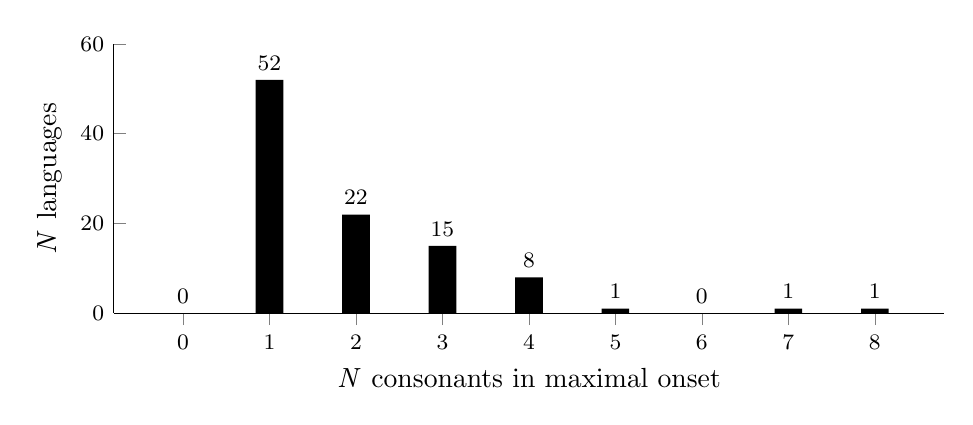
\begin{tikzpicture}
            \begin{axis}[
                    ybar,
                    ylabel={\textit{N} languages},
                    xlabel={\textit{N} consonants in maximal onset},
                    xtick=data,
                    axis lines*=left,
                    ymin=0,
                    ymax=60,
                    scaled y ticks=false,
                    legend pos=north west,
                    ticklabel style={font=\footnotesize\scshape},
                    width=\textwidth,
                    height=5cm,
                    enlarge x limits={0.1},
                    nodes near coords,
                    nodes near coords style={text=black,font=\footnotesize},
                    ]
                \addplot+[
                     fill=black,draw=none
                    ] coordinates {(0,0) (1,52) (2,22) (3,15) (4,8) (5,1) (6,0) (7,1) (8,1)};
\end{axis}
\end{tikzpicture}
\caption{\label{fig:3.1}Maximal onset sizes in sample.}
\end{figure}


\begin{figure}
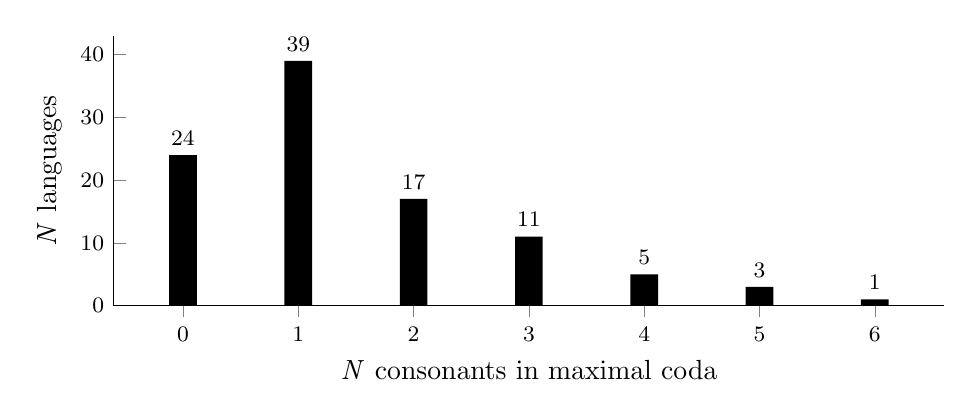
\begin{tikzpicture}
            \begin{axis}[
                    ybar,
                    ylabel={\textit{N} languages},
                    xlabel={\textit{N} consonants in maximal coda},
                    xtick=data,
                    axis lines*=left,
                    ymin=0,
                    scaled y ticks=false,
                    legend pos=north west,
                    ticklabel style={font=\footnotesize\scshape},
                    width=\textwidth,
                    height=5cm,
                    enlarge x limits={0.1},
                    nodes near coords,
                    nodes near coords style={text=black,font=\footnotesize},
                    ]
                \addplot+[
                     fill=black,draw=none
                    ] coordinates {(0,24) (1,39) (2,17) (3,11) (4,5) (5,3) (6,1)};
\end{axis}
\end{tikzpicture}
\caption{\label{fig:3.2}Maximal coda sizes in sample.}
\end{figure}

  The data presented in Figures \ref{fig:3.1} and \ref{fig:3.2} are for onset and coda patterns determined through the procedure described in \sectref{sec:3.2.1}. They do not include the largest word-marginal patterns which occur in languages with syllabic obstruents. There are four languages in the sample which are reported to have syllabic obstruents resulting in Highly Complex patterns at word margins.\footnote{{Additionally, \ili{Tohono O’odham} has syllabic obstruents, but only in independent grammatical particles consisting of a single consonant (determiners and conjunctives). These are not reported to be phonologically bound to adjacent words. Therefore I do not include \ili{Tohono O’odham} in \tabref{tab:3.1}.}} These patterns are presented in \tabref{tab:3.1}, along with the reported maximal onset and coda patterns in the languages.

\begin{table}
\begin{tabular}{lcccc}
\lsptoprule
           &                 &                & \multicolumn{2}{c}{Maximal obstruent string}\\\cmidrule(lr){4-5}
{Language} & {Maximal onset} & {Maximal coda} & word-initial & word-final\\\midrule
\ili{Cocopa} & 4 & 3 & 5 & \phantom{>}3\\
\ili{Semai} & 2 & 1 & 4 & \phantom{>}1\\
\ili{Tashlhiyt} & 1 & 1 & \multicolumn{2}{r}{\textit{(words without vowels)}}\\
\ili{Tehuelche} & 2 & 3 & 3 & >3\\
\lspbottomrule
\end{tabular}
\caption{\label{tab:3.1}Languages in Highly Complex category with syllabic obstruents. Maximal reported onsets and codas are given in first two columns. The sizes of the maximal word-marginal obstruent strings which occur as the result of syllabic obstruents are given in last two columns.}
\end{table}

  In \ili{Tashlhiyt}, the size of maximal word-marginal obstruent strings cannot be determined, because there are many examples of words consisting entirely of obstruents in this language \REF{ex:3.12}. 

\ea\label{ex:3.12}
  \etriple{Tashlhiyt}{Afro-Asiatic}{Morocco}

\textit{tftktstː}

tf.tk.tstː\\
\glt ‘you took it off (\textsc{f})’
\citep[332]{Ridouane2008}
\z

In \ili{Tehuelche}, the reference indicates that sequences of up to six consonants may occur word-finally, but the only illustrative example of a pattern this size given is \REF{ex:3.13}.

\ea\label{ex:3.13}
\etriple{Tehuelche}{Chonan}{Argentina}

\textit{kt͡ʃaʔʃpʃk’n}

k.t͡ʃaʔʃp.ʃ.k’n\\
\glt ‘it is being washed’

(\citealt{FernándezGarayHernández2006}: 13)
\z

This example includes a nasal which may be syllabic (syllable peaks in CC syllables are not marked by the authors). It is clear from the language description that long obstruent sequences come about when syllabic consonants are strung together, but unclear as to what the upper limit on the size of these is. Word-final sequences of at least four obstruents are attested \REF{ex:3.14}.

\ea\label{ex:3.14}
\etriple{Tehuelche}{Chonan}{Argentina}

\textit{maːleʃpʃk’}

maː.leʃp.ʃ.k’\\
\glt ‘they steal’

(\citealt{FernándezGarayHernández2006}: 63)
\z

\subsection{Relationship between onset and coda complexity}\label{sec:3.3.2}

  Here I present an analysis similar to the one presented in \sectref{sec:2.2} for the Complex portion of the \citet{Maddieson2013a} sample. The languages of the sample used in this book are distributed according to their maximal onset and coda patterns.

\begin{table}
\begin{tabular}{l*{2}{r}*{6}{c}}
\lsptoprule
\multicolumn{1}{p{2.25cm}}{Number of Cs\newline in coda} & \multicolumn{8}{c}{Number of Cs in onset}\\\cmidrule(lr){2-9}
 & {One} & {Two} & {Three} & {Four} & {Five} & {Six} & {Seven} & {Eight}\\\midrule
None & 20 & 1 & 2 & 1 & -- & -- & -- & --\\
One & 21 & 12 & 5 & 1 & -- & -- & -- & --\\
Two & 7 & 5 & 5 & -- & -- & -- & -- & --\\
Three & 1 & 4 & 2 & 4 & -- & -- & -- & --\\
Four & 3 & -- & -- & 2 & -- & -- & -- & --\\
Five & -- & -- & -- & -- & 1 & -- & 1 & 1\\
Six & -- & -- & 1 & -- & -- & -- & -- & --\\
\lspbottomrule
\end{tabular}
\caption{\label{tab:3.2}Languages of sample distributed according to maximal onset and coda size.}
\end{table}

Interestingly, it is common for languages with large clusters at one syllable margin to also exhibit large clusters at the other syllable margin in their canonical patterns. Roughly half of languages in the sample which have a maximal cluster of four or more consonants at one syllable margin will have a similarly large maximal cluster at the other syllable margin. It is striking that \textit{all} languages in the sample with maximal onsets of five or more consonants (\ili{Georgian}, \ili{Itelmen}, and \ili{Polish}) also have maximal codas of five consonants. Meanwhile, the bottom left and top right corners of \tabref{tab:3.2} are sparsely populated; that is, there are relatively few languages with very large maximal clusters at one syllable margin and very small maximal clusters (or none at all) at the other margin. A similar pattern can be observed in \tabref{tab:2.2} in \sectref{sec:2.2}, which used a larger sample of 147 languages. Speaking from a strictly distributional point of view, there is no obvious motivation for this pattern. If we consider onset and coda structures to be independent structures, then we would expect to see the full range of possible variation in their combination crosslinguistically. This point will be revisited in \sectref{sec:3.5} and again in \chapref{sec:8}.

\subsection{Syllable structure complexity and obligatoriness of syllable margins}\label{sec:3.3.3}

\citet[336]{Blevins2006} notes another crosslinguistic pattern linking onset and coda structures: languages with only open syllables tend to have optional onsets. In \tabref{tab:3.3} I examine this relationship in the current language sample. There are some languages in which optional onsets may be reported for the canonical syllable structure, but regular and obligatory consonant epenthesis (usually of a glottal stop or fricative) occurs to produce onsets in all ``surface'' forms. In the analysis below, I consider such languages as having obligatory onsets.

\begin{table}
\begin{tabular}{ccc}
\lsptoprule
 \textit{N} languages & Codas occur? & Onset obligatory?\\\midrule
 14 & Y & Y\\
 62 & Y & N\\
 \phantom{1}2 & N & Y\\
 22 & N & N\\
\lspbottomrule
\end{tabular}
\caption{\label{tab:3.3}Languages in sample distributed according to occurrence of codas and obligatoriness of onsets.}
\end{table}

  The relationship reported by Blevins is upheld in the current sample. Of the 24 languages with only open syllables (no codas), only two are reported to have obligatory onsets. Obligatory onsets are more common in languages with coda structures (14/76). The two languages in the sample with obligatory onsets and only open syllables are \ili{Hadza} (Simple) and \ili{Yine} (Highly Complex). It should also be noted that the Oykangand dialect of \ili{Kunjen} used here is reported to have obligatory codas. \ili{Kunjen} is argued to have very marginal onset patterns, with onsets occurring in interjections and sentence-initially in a just a few lexical items (\citealt{Sommer1969,Sommer1970,Sommer1981}, though see \citealt{Dixon1970} for an opposing view).\footnote{{According to Sommer’s analysis, \ili{Kunjen} is a rare example of a language without phonological CV syllables. Another language argued not to have phonological CV syllables is \ili{Arrernte}, a Pama-Nyungan language of central Australia (cf. \citealt{BreenPensalfini1999}), though \citet{Anderson2000} reports a canonical surface syllable structure of (C)(C)V(C) for Western \ili{Arrernte}.}} Therefore \ili{Kunjen} shows a very similar pattern to \ili{Hadza} and \ili{Yine}, except that the syllable margins are reversed.

  The analysis above motivated a more general examination of obligatory syllable margin patterns in the language sample with respect to syllable structure complexity (\tabref{tab:3.4}).

\begin{table}
\begin{tabular}{l *{4}{>{\itshape}c}}
\lsptoprule
& \multicolumn{4}{c}{Syllable structure complexity}\\\cmidrule(lr){2-5}
& \normalfont S & \normalfont MC & \normalfont C & \normalfont HC\\
& \normalfont \textit{N} = 24 & \normalfont \textit{N} = 26 & \normalfont \textit{N} = 25 & \normalfont \textit{N} = 25\\\midrule
{Onset obligatory} & \ili{Hadza}        & \ili{Kambaata}   &  \ili{Koho}   &  \ili{Bench}   \\
                   & \ili{Ute}          &    \ili{Karok}           &      \ili{Lepcha}       &      \ili{Nuu-chah-nulth}\\
                   & \normalfont (2)          &       \ili{Lao}          &      \ili{Mangarrayi}   &           \ili{Semai}\\
                   &              &    \ili{Pacoh}           &    \normalfont(3)            &       \ili{Thompson}\\
                   &              &   \normalfont (4)              &                   &       \ili{Tohono O’odham}\\
                   &              &                    &                   &        \ili{Yakima Sahaptin}\\
                   &              &                    &                   &         \ili{Yine}\\
                   &              &                    &                   &         \normalfont(7)\\
{Coda obligatory}  & -- & -- & -- & \ili{Kunjen} \\
                   &   &   &   & \normalfont (1)\\
\lspbottomrule
\end{tabular}
\caption{\label{tab:3.4}Languages in sample with obligatory syllable margins.}
\end{table}

  Obligatory syllable margins are a minor pattern in the language sample, occurring in only 17 languages, but this feature is most common in languages with Highly Complex syllable structure, occurring in roughly one-third (8/25) of those languages. This feature is least common in languages with Simple syllable structure (2/24 languages). The pattern in the Highly Complex category is statistically significant when compared against the patterns in the other three categories combined ($p = 0.03$ in Fisher’s exact test). This association between syllable structure complexity and obligatoriness of syllable margins has, to my knowledge, not previously been reported.

  Obligatory syllable margins are more common in some areas than others. Five of the languages in \tabref{tab:3.4} are from Southeast Asia \& Oceania. North America is also heavily represented, accounting for another six languages altogether, including four of the languages with obligatory syllable margins from the Highly Complex group. It should further be noted that most of the North American languages with obligatory syllable margins in the Highly Complex group are from the Pacific Northwest (\ili{Nuu-chah-nulth}, \ili{Thompson}, and \ili{Yakima Sahaptin}), so areal factors may be at play. Nevertheless, the Highly Complex pattern in \tabref{tab:3.4} is not entirely areal in nature, as it includes languages from Africa, Southeast Asia \& Oceania, South America, and Australia \& New Guinea. 

  Interestingly, the description of \ili{Itelmen} (Chukotko-Kamchatkan, Highly Complex) suggests that this language, too, had obligatory onsets at some point in its history: morphophonological processes suggest that present-day vowel-initial syllables were at one time initiated by a glottal stop (\citealt{GeorgVolodin1999}: 48).

\subsection{Vocalic nucleus patterns}\label{sec:3.3.4}

  Vocalic nucleus patterns have until now been excluded from the discussion of syllable patterns, as they are not considered in the definitions of syllable structure complexity used here. However, it is important to note that vocalic nucleus patterns can also exhibit different degrees of complexity. In \tabref{tab:3.5} I present a very general analysis of these patterns in the sample, showing the distribution of simple and complex vocalic nuclei by syllable structure complexity.

\begin{table}
\begin{tabular}{lcccc}
\lsptoprule
 & \multicolumn{4}{c}{Syllable Structure Complexity}\\\cmidrule(lr){2-5}
  & S & MC & C & HC\\
  Languages with:     & \textit{N} = 24 & \textit{N} = 26 & \textit{N} = 25 & \textit{N} = 25\\\midrule
 Simple vocalic nuclei only & 12 & \phantom{1}9 & \phantom{1}9 & \phantom{1}9\\
 Complex vocalic nuclei\footnote{\textit{(long vowels, diphthongs, and\slash or vowel sequences)}} & 12 & 17 & 16 & 16\\
\lspbottomrule
\end{tabular}
\caption{\label{tab:3.5}Vocalic nucleus patterns in language sample, by syllable structure complexity.}
\end{table}

  Simple vocalic nuclei -- those consisting of a single short vowel -- occur in every language. The first row of \tabref{tab:3.5} shows the number of languages in each complexity category for which this is the only vocalic nucleus pattern that occurs. Languages in which complex vocalic nuclei occur in addition to simple vocalic nuclei are shown in the second row. For the sake of simplicity I have collapsed three different kind of complex vocalic nucleus patterns in the analysis here. A language is counted as having long vowels if it has contrastive vowel length, but not if it has predictable vowel lengthening, e.g. a longer variant preceding a voiced coda. Diphthongs and tautosyllabic vowel sequences are difficult to disambiguate from one another, as their analyses by different authors may vary; however, vowel sequences reported here as syllable nuclei are those explicitly shown by the author to belong to one syllable, much like a diphthong. That is, this figure does not include cases of hiatus, in which the two vowels in a sequence belong to different syllables.

  \tabref{tab:3.5} shows that complex vocalic nuclei are less likely to occur in languages with Simple syllable structure than in languages from the other categories. This suggests that the potential for more syllable types in languages with more complex syllable structure may be not only a function of larger canonical syllable margins, but also of greater diversity in syllable nucleus patterns. Nevertheless, the analysis above is too coarse to draw strong conclusions about vocalic nucleus patterns and syllable structure complexity. The issue of contrastive vowel length will be treated in greater detail in \chapref{sec:4}, along with contrastive nasalization, voicing, and glottalization patterns in the vowel inventories of the sample.

\subsection{Syllabic consonants}\label{sec:3.3.5}

  In this section I investigate patterns of syllabic consonants in the data. Recall that the previous literature suggests two competing predictions for the relationship between syllable complexity and the presence of syllabic consonants. \citegen{Isačenko1939/1940} phonological typology predicts that ``vocalic'' languages, which tend to have simpler syllable structure, will be more likely to develop syllabic consonants, and specifically syllabic sonorants. Meanwhile, \citet{Bell1978a} notes that syllabic consonants, including syllabic obstruents, often come about through vowel reduction processes, which are also known to produce the clusters characteristic of languages with more complex syllable structure. On the basis of the latter observation, in \sectref{sec:3.1.2} I formulated a hypothesis that languages with more complex syllable structure are more likely to have syllabic consonant patterns.

  Here I analyze languages in which the syllabic consonants are reported as invariant patterns. Most often, the syllabicity of these consonants is predictable from the surrounding consonantal and/or word environment, as illustrated by \REF{ex:3.15}. Less frequently, syllabic consonants are analyzed as separate phonemes which are contrastive with their non-syllabic counterparts (\ref{ex:3.16}a--b).

\ea\label{ex:3.15}
  \etriple{Itelmen}{Chukotko-Kamchatkan}{Russia}

\textit{A word-initial alveolar or bilabial nasal stop preceding another consonant is realized as syllabic.}

/\textbf{m}ɬim/

[\textbf{m̩}ɬim]\\
\glt ‘blood’

(\citealt{GeorgVolodin1999}: 16)
\z

\ea\label{ex:3.16}
  \etriple{Ewe}{Atlantic-Congo}{Ghana, Togo}
\ea   jɔm̩̀
\glt  ‘call me’
\ex kampé
\glt  ‘scissors’
\citep[38]{Ameka1991}
\z
\z

  Three languages are excluded from the current analysis: \ili{Chipaya}, \ili{Nimboran} (both from the Complex category), and \ili{Yine} (from the Highly Complex category). For all three of these languages, there are conflicting reports regarding the occurrence of syllabic consonants, sometimes from the same author.\footnote{{There are a few other languages for which there are suggestions of alternate analyses. The dialect of Sahaptin analyzed here, Yakima, is argued not to have syllabic consonants by \citet{HargusBeavert2006} on the basis of distributional and phonological behavior of consonants in sequences. However, it should be noted that \citet{Minthorn2005} argues for syllabic consonants, including obstruents, in the closely related dialect of Umatilla Sahaptin, on the basis of speaker intuition and acoustic analysis. Additionally, one description of \ili{Alamblak} lists an example of a word consisting entirely of obstruents:} \textrm{\textit{kpt}} \textrm{‘basket type’ \citep[1]{EdmistonEdmiston2003}; however, no further elaboration is given, and obstruents are not included in the description of syllabic consonants in \citet{Bruce1984}, so it is unclear whether syllabic obstruents are an issue of debate for this language. Finally, for \ili{Itelmen}, \citet[42]{Volodin1976} gives transcriptions of lexical items consisting entirely of obstruents (}\textrm{\textit{t͡ʃkpt͡ʃ} }\textrm{‘spoon’). In a later reference, he describes only syllabic sonorants in the language (\citealt{GeorgVolodin1999}).}} For example, Matteson gives the following description for \ili{Yine}, which seems to suggest that consonants in complex onsets both belong to a syllable with a vocalic nucleus and are simultaneously themselves syllabic:

\begin{quote}
“We number the consonants of the syllable, beginning with the consonant that immediately precedes the nuclear vowel: +C\textsuperscript{3} +C\textsuperscript{2} +C\textsuperscript{1}V. In the positions of consonants C\textsuperscript{2} and C\textsuperscript{3} occur syllabic allophones of the consonants. Thus the syllable is a complex unit consisting of from one to three syllabic units.” 
\citep[23]{Matteson1965}
\end{quote}

Because of the conflicting descriptions of these languages, I opted to exclude them from the current analysis. \ili{Georgian} and \ili{Tashlhiyt} also have conflicting descriptions with respect to the occurrence of syllabic consonants, but in both of these cases experimental evidence has been presented to support one analysis over another. The articulatory and acoustic experiments in \citet{Ridouane2008} and \citet{GoldsteinEtAl2007} support a syllabic consonant analysis for \ili{Tashlhiyt}, while native speaker intuition reported in \citet{Chitoran1999} does not support an analysis of syllabic sonorants for \ili{Georgian}. It is interesting to note that all of the languages with conflicting descriptions -- those discussed here and the ones mentioned in footnote 6 -- are from the Complex and Highly Complex categories. This recalls the observation noted previously, in which transitions in consonant clusters on the one hand and syllabic consonants on the other may have similar motivations and acoustic manifestations.

\begin{table}
\begin{tabular}{lcccc}
\lsptoprule
 & \multicolumn{4}{c}{Syllable Structure Complexity}\\\cmidrule(lr){2-5}
                        & S & MC & C & HC\\
  Languages with:       &  \textit{N} = 24   & \textit{N} = 26                & \textit{N} = 23     & \textit{N} = 24\\\midrule

 Syllabic consonants\\
   of any kind                         & \textbf{2} & \textbf{6} & \textbf{5} & \textbf{11}\\
 \textit{Syllabic nasals} & 2 & 5 & 5 & 10\\
 \textit{Syllabic liquids} & -- & 2 & 1 & 6\\
 \textit{Syllabic obstruents} & -- & -- & -- & 5\\
 No syllabic\\
    consonants            & \textbf{22} & \textbf{20} & \textbf{18} & \textbf{13}\\
\lspbottomrule
\end{tabular}
\caption{\label{tab:3.6}Presence of invariant syllabic consonants in language sample, by syllable structure complexity. Chipaya (Complex), Nimboran (Complex), and Yine (Highly Complex) excluded.}
\end{table}

  The syllabic consonant patterns reported for the languages of the sample can be found in \tabref{tab:3.6}. There is a steadily increasing trend in the proportion of languages with these patterns as syllable structure complexity increases: only two of languages with Simple syllable structure are reported to have syllabic consonants, compared to 11 of the languages in the Highly Complex category. The trend in the Highly Complex category is statistically significant when compared to the trends in the other three categories combined ($p = 0.01$ in Fisher’s exact test). 
  
  Examining the particular kinds of syllabic consonants represented, the patterns are similar to what is reported in \citet{Bell1978a}. Most languages with syllabic consonants have syllabic nasals, and languages with syllabic obstruents are rare. While languages from all four categories have syllabic nasals and most have syllabic liquids, syllabic obstruents are only reported for languages in the Highly Complex category. This is not a remnant of the way the Highly Complex category is defined: recall that languages with syllabic obstruents are categorized as Highly Complex only if these structures participate in word-marginal sequences of three obstruents or more. It is striking that no languages with simpler syllable structure are reported to have syllabic obstruents. Even if the three languages excluded from the previous analysis were included here, the distribution of syllabic obstruents would be among two languages with Complex syllable structure and six languages with Highly Complex syllable structure. 

  It should also be noted that three of the languages with syllabic obstruents (\ili{Cocopa}, \ili{Semai}, \ili{Tashlhiyt}) are reported to also have both syllabic nasals and syllabic liquids. \ili{Tehuelche} does not have syllabic liquids. \ili{Tohono O’odham} is the only language which has syllabic obstruents but not syllabic sonorant consonants. This indicates that the trend in \tabref{tab:3.6} -- by which Highly Complex languages are more likely than any of the other categories to have syllabic consonants  -- is not driven by the inclusion of syllabic obstruents in the definition of that category, or skewed by potential misanalyses which confound syllabic obstruents and large tautosyllabic clusters. The trend can be obtained from the syllabic nasal and liquid patterns in the sample.

  While the analyses presented above are for the invariant syllabic consonant patterns observed in the sample, there were also several cases in which syllabic consonants were reported to occur in variation with CV or VC sequences, as illustrated by \xxref{ex:3.17}{ex:3.18}.

\ea\label{ex:3.17}
\etriple{Sichuan Yi}{Sino-Tibetan}{China}

\textit{Nasals and laterals preceding [ɨ] occur in free variation with syllabic consonants.}

/lɨ/

[lɨ]{\textasciitilde}[{\fontspec{LibertinusSerif-Regular.otf}[Path=\fontpath,FakeBold=1.5] l̩}]
\citep[31]{Gerner2013}
\z

\ea\label{ex:3.18}
   \etriple{Mamaindê}{Nambiquaran}{Brazil}

\textit{When an unstressed vowel is lost resulting in a sequence of nasal plus consonant, a preceding nasal becomes syllabic.}

/ˈjohnalatʰawa/

[ˈjoh\textbf{n̩}latʰwa]\\
\glt ‘it is low’
\citep[262--263]{Eberhard2009}
\z

\begin{table}
\begin{tabular}{lcccc}
\lsptoprule
 & \multicolumn{4}{c}{Syllable Structure Complexity}\\\cmidrule(lr){2-5}
 Languages with  & S & MC & C & HC\\
   variable:     &   \textit{N} = 1 & \textit{N} = 3 &  \textit{N} = 2 & \textit{N} = 3\\\midrule
 \textit{Syllabic nasals}     & 1 & 3 & 2 & 3\\
 \textit{Syllabic liquids}    & 1 & -- & -- & 2\\
 \textit{Syllabic obstruents} & -- & 1 & -- & 1\\
\lspbottomrule
\end{tabular}
\caption{\label{tab:3.7}Distribution of languages in sample with syllabic nasals, liquids, and obstruents occurring in variation with VC or CV structures.}
\end{table}

  \tabref{tab:3.7} shows the distribution of variable processes producing syllabic consonants in the data. Though the data set is very small, it is interesting that the general distributional pattern is similar to that presented in \tabref{tab:3.6}. The occurrence of syllabic consonants in variation with VC or CV structures is least frequent among languages with Simple syllable structure, and in all categories nasals are the most common syllabic consonant to result. Variable syllabic obstruents occur in two languages. In \ili{Paiwan} (Moderately Complex), syllabic obstruents may occur when schwa is reduced immediately after a sibilant in rapid speech, and in \ili{Kabardian} (Highly Complex), they occur as the result of an optional process of high vowel contraction (\ref{ex:3.19}--\ref{ex:3.20}):

\ea\label{ex:3.19}
  \etriple{Paiwan}{Austronesian}{Taiwan}

/səkam/

[səkam]{\textasciitilde}[\textbf{s̩}kam]\\
\glt ‘mattress’
\citep[41]{Chang2006}
\z

\ea\label{ex:3.20}
  \etriple{Kabardian}{Abkhaz-Adyge}{Russia, Turkey}

/ɬ{}'əʒ/

[ɬ’iʒ]{\textasciitilde}[ɬ{}'\textbf{ʒ̩}]\\
\glt ‘old man’
\citep[24]{Kuipers1960}
\z

\ili{Kabardian} is also the only language in the sample reported to have both invariant syllabic consonants (for sonorants in certain consonant environments) and variable syllabic consonants as a result of synchronic phonetic processes like the one illustrated above.

  Returning to the hypothesis stated at the beginning of this section, there is evidence that languages with more complex syllable structure are more likely to have syllabic consonant patterns. Specifically, languages with Highly Complex syllable structure are the most likely of all those in the sample to have invariant syllabic consonants, while languages with Simple syllable structure are the least likely. Variable processes resulting in syllabic consonants are also relatively more frequent in languages with non-Simple syllable structure.

\subsection{Morphological patterns}\label{sec:3.3.6}

  In this section I analyze the morphological patterns associated with syllable patterns in the language sample. First, I report the morphological constituency patterns observed in the maximal onset and coda structures in each language. Then I present an analysis of the kinds of morphemes (lexical or grammatical) in which syllabic consonants in the language sample occur. I test the hypotheses formulated in \sectref{sec:3.1.2} with respect to these patterns: first, that as syllable structure complexity increases, so does the likelihood that the largest syllable margin types in a language will be morphologically complex; and second, that as syllable structure complexity increases, so does the likelihood that syllabic consonants occurring in a language will belong to grammatical elements.

  Since morphologically complex instances of syllable patterns are often not explicitly described and must be gathered from the examples, it was impractical and in many cases impossible to find morpheme-internal and morphologically complex instances of the same specific consonant sequence in each language, especially for the larger clusters. The patterns analyzed here are for the maximal onset and coda \textit{types}, e.g. CC. For example, the maximal coda in \ili{Gaam} is two consonants. The word-final patterns shown in the examples below would be taken as evidence that the maximal coda occurs in both morpheme-internal (\ref{ex:3.21}a) and morphologically complex (\ref{ex:3.21}b) contexts.

\ea\label{ex:3.21}
\etriple{Gaam}{Eastern Jebel}{Sudan}

\ea  bāɡd̪à\textbf{rs}\\
\glt ‘lizard type’
\ex  ɡəū\textbf{r-d̪}\\
stomach-\textsc{sg}\\
\glt ‘stomach’
(\citealt{Stirtz2011}: 32, 37)
\z
\z

  Note also that the definition of \textit{morphologically complex} here refers to sequences derived by any morphological process. That is, sequences derived through reduplication or nonconcatenative processes such as subtractive morphology are also considered to be morphologically complex, even though they don’t involve more than one distinct morpheme.

  First I test \citegen{Greenberg19651978} prediction in the data: as the size of a syllable margin increases, so does the probability that it contains morpheme boundaries. Figures \ref{fig:3.3} and \ref{fig:3.4} show morphological constituency patterns in maximal onset and coda types in the data.

  
\begin{figure}
\begin{tikzpicture}
\pgfplotstableread{data/fig33.csv}{\table}
    \pgfplotstablegetcolsof{\table}
    \pgfmathtruncatemacro\numberofcols{\pgfplotsretval-1}
            \begin{axis}[easterdaystacked,
                                xticklabel style={align=center},
                                xticklabels={CC,CCC,CCCC,{CCCCC\\or more}},
                        ]
            \foreach \i in {1,...,\numberofcols} {
                \addplot+[
                    /pgf/number format/read comma as period, fill
                    ] table [x index={1},y index={\i},x expr=\coordindex] {\table};
                \pgfplotstablegetcolumnnamebyindex{\i}\of{\table}\to{\colname} % Adding column headers to legend
                \addlegendentryexpanded{\colname}
            }
            \end{axis}                                                                           
\end{tikzpicture}
\caption{\label{fig:3.3}Morphological constituency patterns in maximal onset types in data. For each maximal onset type, figure shows proportion of languages exhibiting the given morphological patterns for that type.}
\end{figure}


\begin{figure}
\begin{tikzpicture}
\pgfplotstableread{data/fig34.csv}{\table}
    \pgfplotstablegetcolsof{\table}
    \pgfmathtruncatemacro\numberofcols{\pgfplotsretval-1}
            \begin{axis}[easterdaystacked,
                                xticklabel style={align=center},
                                xticklabels={CC,CCC,CCCC,{CCCCC\\or more}},
                        ]
            \foreach \i in {1,...,\numberofcols} {
                \addplot+[
                    /pgf/number format/read comma as period, fill
                    ] table [x index={1},y index={\i},x expr=\coordindex] {\table};
                \pgfplotstablegetcolumnnamebyindex{\i}\of{\table}\to{\colname} % Adding column headers to legend
                \addlegendentryexpanded{\colname}
            }
            \end{axis}                                                                           
\end{tikzpicture}
\caption{\label{fig:3.4}Morphological constituency patterns in maximal coda types in data. For each maximal coda type, figure shows proportion of languages exhibiting the given morphological patterns for that type.}
\end{figure}

  For both maximal onset and maximal coda patterns in the data, the proportion of languages having these clusters solely in morphologically complex contexts increases with cluster size. However, morphologically complex patterns also occur alongside morpheme-internal patterns in the maximal margins for a number of languages (the “Both patterns” trend in Figures \ref{fig:3.3} and \ref{fig:3.4}). When this trend is additionally considered, we find that maximal coda cluster types are generally more likely than maximal onset types to exhibit morphologically complex patterns. We also find that all maximal cluster types of five consonants or larger are found only in morphologically complex contexts.

  Interestingly, there are some language-internal patterns in the data which go against Greenberg’s prediction. In \ili{Lelepa} there are biconsonantal onsets showing both morphological patterns, but the only attested triconsonantal onsets are within morphemes (\ref{ex:3.22}a--c).

\ea\label{ex:3.22}
\etriple{Lelepa}{Austronesian}{Vanuatu}

\ea  n-maloɡo\\
\textsc{nmlz}-darken\\
\glt ‘darkness’

\ex  nmal\\
\glt ‘trunk’

\ex  psruki\\
\glt ‘speak’

(\citealt{Lacrampe2014}: 107, 207, 42)
\z
\z

  The analyses presented in Figures \ref{fig:3.3}--\ref{fig:3.4} test Greenberg’s specific predictions regarding cluster size. However, the hypothesis in (\ref{ex:3.4}a) is formulated with respect to syllable structure complexity, which is a slightly different question, though we expect to find a similar pattern due to how the categories are defined. In Figures \ref{fig:3.5}--\ref{fig:3.6} I present the morphological constituency patterns observed by syllable structure complexity category. Note that these figures only include the languages from each category which have complex onsets or complex codas, respectively.


\begin{figure}
\begin{tikzpicture}
\pgfplotstableread{data/fig35.csv}{\table}
    \pgfplotstablegetcolsof{\table}
    \pgfmathtruncatemacro\numberofcols{\pgfplotsretval-1}
            \begin{axis}[easterdaystacked,
                                xticklabels={{MC}, C, {HC}},
                        ]
            \foreach \i in {1,...,\numberofcols} {
                \addplot+[
                    /pgf/number format/read comma as period, fill
                    ] table [x index={1},y index={\i},x expr=\coordindex] {\table};
                \pgfplotstablegetcolumnnamebyindex{\i}\of{\table}\to{\colname} % Adding column headers to legend
                \addlegendentryexpanded{\colname}
            }
            \end{axis}                                                                           
\end{tikzpicture}
\caption{\label{fig:3.5}Morphological constituency patterns in maximal complex onsets, by syllable structure complexity category. For each category, the figure shows the proportion of languages exhibiting the given morphological patterns in its complex onsets.}
\end{figure}


\begin{figure}
\begin{tikzpicture}
\pgfplotstableread{data/fig36.csv}{\table}
    \pgfplotstablegetcolsof{\table}
    \pgfmathtruncatemacro\numberofcols{\pgfplotsretval-1}
            \begin{axis}[easterdaystacked,
                                xticklabels={C, {HC}},
                                enlarge x limits={0.7}
                        ]
            \foreach \i in {1,...,\numberofcols} {
                \addplot+[
                    /pgf/number format/read comma as period, fill
                    ] table [x index={1},y index={\i},x expr=\coordindex] {\table};
                \pgfplotstablegetcolumnnamebyindex{\i}\of{\table}\to{\colname} % Adding column headers to legend
                \addlegendentryexpanded{\colname}
            }
            \end{axis}                                                                           
\end{tikzpicture}
\caption{\label{fig:3.6} Morphological constituency patterns in maximal complex codas, by syllable structure complexity category. For each category, the figure shows the proportion of languages exhibiting the given morphological patterns in its complex onsets. Note that the one language with complex codas from the Moderately Complex category -- Eastern Khanty -- is not included in the figure. Its very marginal complex codas are always morphologically complex.}
\end{figure}


  The figures show that as syllable structure complexity increases, both maximal onset and maximal coda clusters are more likely to have morphologically complex patterns, confirming the hypothesis in (\ref{ex:3.4}a).

  The patterns in Figures~\ref{fig:3.5}--\ref{fig:3.6} are combined in \figref{fig:3.7} in order to show the general trend for morphologically complex patterns in maximal syllable-mar\-gin\-al clusters with respect to syllable structure complexity in the language sample. In this figure onset and coda patterns are collapsed, and the “both contexts” and “only morphologically complex” patterns are combined. For each category, the figure shows the percentage of languages with complex syllable margins for which morphologically complex patterns occur in either or both maximal syllable margins.


\begin{figure}  
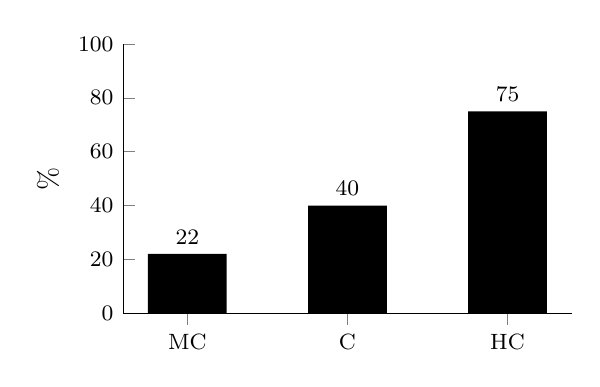
\begin{tikzpicture}
            \begin{axis}[
                    ybar,
                    ylabel={\%},
                    xtick=data,
                    axis lines*=left,
                    ymin=0,
                    ymax=100,
                    legend pos=north west,
                    ticklabel style={font=\footnotesize},
                    width=.6\textwidth,
                    enlarge x limits={.2},
                    height=5cm,
                    bar width=1cm,
                    nodes near coords,
                    nodes near coords style={text=black,font=\footnotesize},
                    xticklabels={{MC}, C, {HC}},
                    ]
                \addplot+[
                     fill=black,draw=none
                    ] coordinates {(0,22) (1,40) (2,75)};
\end{axis}
\end{tikzpicture}
\caption{\label{fig:3.7} Percentage of languages in each category exhibiting morphologically complex patterns in either or both of its maximal syllable margins.}
\end{figure}

  Morphologically complex patterns can be found in the maximal syllable margins of most languages from the Highly Complex category, and this pattern is statistically significant when compared against the patterns in the other two categories combined ($p < 0.01$ in Fisher’s exact test). However, there are six languages in this category for which I could determine only morpheme-internal patterns. In \ili{Wutung}, the maximal margin is explicitly described as occurring within a few apparently single-morpheme lexical items. In \ili{Kunjen} and \ili{Lezgian}, maximal coda and onset clusters, respectively, seem to be limited to single-morpheme lexical items, though the references consulted do not explicitly state this. In \ili{Menya}, the only morphologically complex instance of a maximal cluster that could be found was in an abstract phonemic transcription for which the phonetic form was unclear. In \ili{Passamaquoddy-Maliseet}, examples of morphologically complex instances of maximal clusters could not be found, though it seems as though the morphology could produce them. The remaining language, \ili{Semai}, has syllabic consonants and will be discussed below.

  Recall that there are four languages in the Highly Complex portion of the sample for which the largest word-marginal obstruent sequences include syllabic consonants. The maximal ``true'' onset/coda clusters reported for these languages (cf. \tabref{tab:3.2}) were included in the previous analyses in this section, but the maximal word-marginal sequences were not. I present the morphological patterns for these sequences in \tabref{tab:3.8}.

\begin{table}
\begin{tabular}{lcccc}
\lsptoprule
{Language}& {Maximal \#\_} & {Morphol.} & Maximal \_\#  & Morphol. \\
          &   obstruent string     &      pattern                   &  obstruent string   &      pattern                \\\midrule
\ili{Cocopa}    & 5                      & complex & 3                      & complex\\
\ili{Semai}     & 4                      & complex & 1                      & --\\
\ili{Tashlhiyt} & --\footnote{(words without vowels)} & complex & --\textsuperscript{\itshape a} & complex\\
\ili{Tehuelche} & 3                      & complex & >3                     & complex\\
\lspbottomrule
\end{tabular}
\caption{\label{tab:3.8}Morphological patterns of maximal word-marginal obstruent sequences in languages with syllabic obstruents in Highly Complex category.}
\end{table}

  All of the maximal word-marginal obstruent sequences in the languages in \tabref{tab:3.8} occur in morphologically complex contexts. For example, in \ili{Semai}, all maximal word-initial consonant sequences, and indeed all word-initial sequences of more than two consonants, are derived through reduplication processes \REF{ex:3.23}.

\ea\label{ex:3.23}
  \etriple{Semai}{Austroasiatic}{Malaysia}

ɡp.ɡ.hup (< ɡhup )\\
\glt ‘irritation on skin (e.g. from bamboo hair)’

(\citealt{Sloan1988}: 320; \citealt{Diffloth1976a}: 256)
\z

Though maximal word-marginal obstruent string length cannot be determined in \ili{Tashlhiyt} due to the occurrence of many words consisting entirely of obstruents in this language, the longest such words are morphologically complex \REF{ex:3.24}.

\ea\label{ex:3.24}
  \etriple{Tashlhiyt}{Afro-Asiatic}{Morocco}

t-sː-kʃf-t=stː

ts.sk.ʃf.tstː\\
\glt ‘you dried it (\textsc{f})’

(\citealt{Ridouane2008}: 332; interlinear gloss not provided)
\z

  Now we turn to the hypothesis in (\ref{ex:3.4}b): as syllable structure complexity increases, so does the likelihood that syllabic consonants occurring in a language will belong to grammatical elements. This is based partly on \citegen{Bell1978a} observation that the syllabic consonants in his typological survey were often restricted to grammatical particles and affixes.

  Only the languages reported in \sectref{sec:3.3.5} as having invariant syllabic consonant patterns are included in the analysis here. Additionally, \ili{Kabardian} is excluded from the present analysis because its precise patterns could not be determined. For each kind of syllabic consonant analyzed (nasal, liquid, and obstruent), I determine whether that type occurs in lexical morphemes, grammatical morphemes, or both. For example, in \ili{Bench}, syllabic nasals can be found in both lexical and grammatical morphemes \REF{ex:3.25}.

\ea\label{ex:3.25}
  \etriple{Bench}{Ta-Ne-Omotic}{Ethiopia}

\ea   ɡȕp\textbf{\={m}}\\
\glt ‘foam’

\ex   njāʔ-\textbf{\={n}}d

child-\textsc{pl}\\
\glt ‘children’

(\citealt{Rapold2006}: 107, 111)
\z
\z

  In Tables \ref{tab:3.9}--\ref{tab:3.11} I present analyses for the morphological patterns of each kind of syllabic consonant (nasal, liquid, and obstruent) observed in the data.

\begin{table}
\begin{tabular}{lcccc}
\lsptoprule
 & \multicolumn{4}{c}{Syllable structure complexity}\\\cmidrule(lr){2-5}
Languages with & S & MC & C & HC\\
syllabic nasals in: & \textit{N} = 2 & \textit{N} = 5 & \textit{N} = 6 & \textit{N} = 9\\\midrule
 \textit{Lexical morphemes only} & 1 & 3 & 2 & 1\\
 \textit{Lex. and gram. morphemes} & -- & 2 & 2 & 6\\
\textit{Gram. morphemes only} & 1 & -- & 2 & 2\\
\lspbottomrule
\end{tabular}
\caption{\label{tab:3.9}Morphological patterns of syllabic nasals in sample, by syllable structure complexity. Kabardian (Highly Complex) is omitted as its pattern could not be determined.}
\end{table}




\begin{table}
\begin{tabular}{lcccc}
\lsptoprule
 & \multicolumn{4}{c}{Syllable structure complexity}\\\cmidrule(lr){2-5}
Languages with & S & MC & C & HC\\
syllabic liquids in: & \textit{N} = 0 & \textit{N} = 2 & \textit{N} = 1 & \textit{N} = 5\\\midrule
 \textit{Lexical morphemes only} & -- & 2 & 1 & 2\\
 \textit{Lex. and gram. morphemes} & -- & -- & -- & 2\\
\textit{Gram. morphemes only} & -- & -- & -- & 1\\
\lspbottomrule
\end{tabular}
\caption{\label{tab:3.10}Morphological patterns of syllabic liquids in sample, by syllable structure complexity. Kabardian (Highly Complex) is omitted as its pattern could not be determined.}
\end{table}


\begin{table}
\begin{tabular}{lcccc}
\lsptoprule
 & \multicolumn{4}{c}{Syllable structure complexity}\\\cmidrule(lr){2-5}
Languages with & S & MC & C & HC\\
syllabic obstruents in: & \textit{N} = 0 & \textit{N} = 0 & \textit{N} = 0 & \textit{N} = 5\\\midrule
 \textit{Lexical morphemes only} & -- & -- & -- & --\\
 \textit{Lex. and gram. morphemes} & -- & -- & -- & 1\\
 \textit{Grammatical} \\
\textit{morphemes only} & -- & -- & -- & 4\\
\lspbottomrule
\end{tabular}
\caption{\label{tab:3.11}Morphological patterns of syllabic obstruents in sample, by syllable structure complexity.}
\end{table}

  In general, the pattern by which syllabic consonants are found to occur in grammatical morphemes, either exclusively or in addition to lexical morphemes, is the dominant one in the data. This is the case for 15/22 languages with syllabic nasals and all of the languages with syllabic obstruents, though this trend does not hold for languages with syllabic liquids. Within this very small data set, the trend also appears to increase with syllable structure complexity, suggesting support for the hypothesis. 

  In fact most of the languages with syllabic consonants in the Highly Complex category have these sounds in grammatical items. In \ili{Tehuelche}, for example, \textit{all} syllabic consonants correspond to or belong to grammatical morphemes \REF{ex:3.26}.

\ea\label{ex:3.26}
\etriple{Tehuelche}{Chonan}{Argentina}

k.t͡ʃaʔʃp.ʃ.k’n

k-t͡ʃaʔʃp-ʃ-k’n

\textsc{refl}-wash-\textsc{ps-realis}\\
\glt ‘it is being washed’

(\citealt{FernándezGarayHernández2006}: 13)
\z

  To summarize, in this section the morphological patterns of maximal onset types, maximal coda types, and syllabic consonant inventories in the sample have been examined. In both cases there is support for the hypotheses in \REF{ex:3.4}. Clearly morphology contributes an important role to the development of complex syllable patterns. While this point will be only briefly revisited in the discussion in \sectref{sec:3.5}, it will be discussed in further detail in \chapref{sec:8}.

\section{Properties of highly complex syllable structure}\label{sec:3.4}

  Having described the general patterns of maximal onsets, maximal codas, and syllabic consonants in the data, I now turn to an examination of the properties of syllable structure in the languages in the Highly Complex portion of the sample. In \sectref{sec:3.4.1} I give examples of the syllable patterns occurring in each of these languages. In \sectref{sec:3.4.2} I attempt to characterize the prevalence of Highly Complex structures within each of the languages by examining restrictions on consonant combinations and reported frequency patterns. In \sectref{sec:3.4.3} I present information on the acoustic and perceptual properties of Highly Complex structures.

\subsection{Examples of Highly Complex syllable patterns in sample}\label{sec:3.4.1}

  In order to provide a better picture of what specific syllable patterns occur in the languages of the Highly Complex portion of the sample, I list some representative structures in \tabref{tab:3.12}. The definition of Highly Complex syllable structure includes any onset or coda structure of three obstruents, or of four consonants or more in length. It also includes any word-marginal sequence containing syllabic obstruents such that a sequence of three or more obstruents occurs at a word margin. For each language I give a set of examples for each onset, coda, and/or word-marginal cluster that occurs at each of the following lengths: three consonants, four consonants, and five or more consonants. For \ili{Tashlhiyt}, I have given some examples of vowelless words in the rightmost column, but have not assigned them to a word margin.

{\footnotesize\begin{longtable}{llll}
\caption{\label{tab:3.12}Representative sample of Highly Complex patterns occurring in data. (--) indicates that there are no reported patterns of this kind in the given language. The Yine patterns are in parentheses because they are representative triconsonantal clusters for the language but do not contain three obstruents (see discussion in \sectref{sec:3.2.3}).}\\
\lsptoprule  & \multicolumn{3}{c}{Highly Complex structures}\\\cmidrule(lr){2-4} {Language} & 3-obstruent & 4-C & 5-C and larger\\\midrule\endfirsthead\midrule Language & 3-obstruent & 4-C & 5-C and larger\\\midrule\endhead
\lspbottomrule\endlastfoot\endfoot
{Alamblak} & \textbf{O:} tkb & -- & --\\
{Bench} & \textbf{Cd:} pst & -- & --\\
{Menya} & \textbf{O:} tpq, ptq & -- & --\\
{Kabardian} & \textbf{O:} zbɣ, pɕt, psk’ & -- & --\\
{Lezgian} & \textbf{O:} ʃtk, kst, ktk & -- & --\\
{Yine} & \textbf{O:} (pcɾ, nt͡sp, nt͡ʃk) & -- & --\\
{Camsá} & \textbf{O:} stx, st͡ʃb, sʃt͡s & {\textbf{O:} ɸstx} & -- \\
{Semai} & \textbf{\#\_:} st.s & \textbf{\#\_:} ɡp.ɡ.h & --\\
{Nuu-chah-} & \textbf{Cd:} t͡ʃtq, kqs, qt͡ɬs, tħt͡s & \textbf{Cd:} mtqʃ, ħsqħ, nkqħ & --\\
nulth \\\tablevspace
{Wutung} & -- & \textbf{O:} hmbl & --\\
{Doyayo} & -- & \textbf{Cd:} βlts, ɣldz, mnts & --\\
{Kunjen} & -- & \textbf{Cd:} lbmb, ɹdnd, jɡŋɡ & --\\
{Passama-} & \textbf{O:} psk, ksp, pskʷ & -- & --\\
quoddy-  &  \textbf{Cd:} pskʷ, kskʷ  \\
Maliseet \\\tablevspace
{Qawasqar} & \textbf{O:} qsq, qst, qsk & \textbf{O:} qsqj & --\\
           & \textbf{Cd:} qsq  \\
{Tehuelche} & \textbf{\#\_:} kʃ.x, kʃ.ʔ  & \textbf{\_\#:} ʃp.ʃ.k’ & --\\
            & \textbf{Cd:} ʔʃp\\
{Albanian} & \textbf{O:} skt, pʃt & \textbf{O:} t͡ʃmpl, zmbr & --\\
            & \textbf{Cd:} pʃt, kst  \\
{Mohawk} & \textbf{O:} ksk, kts, kst, kht  & \textbf{O:} shnj, khnj & --\\
            & \textbf{Cd:} ʔks, ʔts, kst \\
{Yakima} & \textbf{O:} pʃχ, tkʷs, q’ʃp  & \textbf{O:} ʃtχn, ksks   & --\\
Sahaptin &  \textbf{Cd:} tks, stk, pt͡ɬ’k & \textbf{Cd:} wtkʷʃ, wq’χʃ, jlps\\\tablevspace
{Tohono} & \textbf{Cd:} ɡʂp, tpk, bst͡ʃ, psk & \textbf{O:} ndʂʔ & --\\
O’odham & & \textbf{Cd:} ʃt͡ʃkt͡ʃ, t͡ʃspk, ɡʂsp\\\tablevspace
{Polish} & \textbf{O:} pʃt, xʃt, tkfʲ  & \textbf{O:} pstʃ, fksʃ, vzɡl  & \textbf{O:} spstr \\
            & \textbf{Cd:} psk, stf, ʃt͡ʃp & \textbf{Cd:} ɲstf, tstf, rstf, pstf & \textbf{Cd:} mpstf\\
{Thompson} & \textbf{O:} spt, st͡s’k  & \textbf{Cd:} t͡sxst͡s, jxst͡s, ɬkst & \textbf{Cd:} ɬqsxtxʷ\\
           & \textbf{Cd:} xʷkt, xʷst͡s, pst͡s\\
{Itelmen} & \textbf{O:} kth, kp'k', ɬqz  & \textbf{O:} ttxn, ksxw, ktxl  & \textbf{O:} kpɬkn, tksxqz, kstk’ɬkn \\
            & \textbf{Cd:} pɬh, sht & \textbf{Cd:} nt͡ʃpx, mpɬx, ɬtxt͡ʃ & \textbf{Cd:} nxɬxt͡ʃ, mstxt͡ʃ\\
{Georgian} & \textbf{O:} t'k'b, p't͡s'k', psk’ & \textbf{O:} txzβ̞, t͡s’q’ɾt, brt͡s'q{}'  & \textbf{O:} p’ɾt͡s’k’β̞, ɡβ̞pɾt͡skβ̞n \\
            & & \textbf{Cd:} ɾtxl, ɾt'q'l, nt͡ʃxl & \textbf{Cd:} nt͡ʃxls, ɾt͡s’q’β̞s, ɾt'k'ls\\
{Cocopa} & \textbf{O:} sxʈ, pskʷ, xps  & \textbf{O:} ʂt͡ʃxʔ, pʂt͡ʃʔ& \textbf{\#\_:} pk.ʃkw\\
            & \textbf{Cd:} qsk, ʂsk, xsk  & \textbf{\#\_:} p.t͡ʃx.m \\
{Tashlhiyt} & \textbf{\#\_:} ts.t  & \textbf{\#\_:} ts:χs  & (\textbf{V-less wds:}) tsːftχt,\\
            & \textbf{\_\#:} kʷtt, ʃ.kd & \textbf{\_\#:} ststː & \hspace{2em} tftktstː, tsːkʃftstː\\ 
\end{longtable}}

% % % \begin{table} % Joined with the Table above (author's request)
% % % \begin{tabular}{llll}
% % % \lsptoprule
% % %  & \multicolumn{3}{c}{Highly Complex structures}\\\cmidrule(lr){2-4}
% % % {Language} & {3-obstruent} & {4-C} & {5-C and larger}\\\midrule
% % % {Thompson} & \textbf{Onset:} spt, st͡s’k  & \textbf{Coda:} t͡sxst͡s, jxst͡s, ɬkst & \textbf{Coda:} ɬqsxtxʷ\\
% % %            & \textbf{Coda:} xʷkt, xʷst͡s, pst͡s\\
% % % {Itelmen} & \textbf{Onset:} kth kp'k' ɬqz  & \textbf{Onset:} ttxn, ksxw, ktxl  & \textbf{Onset:} kpɬkn, tksxqz, kstk’ɬkn \\
% % %             & \textbf{Coda:} pɬh sht & \textbf{Coda:} nt͡ʃpx, mpɬx, ɬtxt͡ʃ & \textbf{Coda:} nxɬxt͡ʃ, mstxt͡ʃ\\
% % % {Georgian} & \textbf{Onset:} t'k'b p't͡s'k' psk’ & \textbf{Onset:} txzβ ̞, t͡s’q’ɾt, brt͡s'q{}'  & \textbf{Onset:} p’ɾt͡s’k’β ̞, ɡβ ̞pɾt͡skβ ̞n \\
% % %             & & \textbf{Coda:} ɾtxl, ɾt'q'l, nt͡ʃxl & \textbf{Coda:} nt͡ʃxls, ɾt͡s’q’β ̞s, ɾt'k'ls\\
% % % {Cocopa} & \textbf{Onset:} sxʈ, pskʷ, xps  & \textbf{Onset:} ʂt͡ʃxʔ pʂt͡ʃʔ, p.t͡ʃx.m & \textbf{Word-initial:} pk.ʃkw\\
% % %             & \textbf{Coda:} qsk, ʂsk, xsk \\
% % % {Tashlhiyt} & \textbf{Word-initial:} ts.t  & \textbf{Word-initial:} ts:χs  & (\textbf{Words without vowels:)} tsːftχt, tftktstː, tsːkʃftstː\\
% % %             & \textbf{Word-final:} kʷtt, ʃ.kd & \textbf{Word-final:} ststː \\
% % % \lspbottomrule
% % % \end{tabular}
% % % \caption{\label{tab:3.12cont}Representative sample of Highly Complex patterns occurring in data. (--) indicates that there are no reported patterns of this kind in the given language. The Yine patterns are in parentheses because they are representative triconsonantal clusters for the language but do not contain three obstruents (see discussion in \sectref{sec:3.2.3}).}
% % % \end{table}

  The languages in \tabref{tab:3.12} are organized so as to highlight several coherent patterns in the data. In the first set of languages (\ili{Alamblak}, \ili{Bench}, \ili{Menya}, \ili{Kabardian}, \ili{Lezgian}, \ili{Yine}, \ili{Camsá}, \ili{Semai}, and \ili{Nuu-chah-nulth}), Highly Complex patterns are limited to one syllable or word margin, usually the onset/initial context. The Highly Complex patterns in these languages are typically limited to triconsonantal clusters, though four-consonant clusters occur in \ili{Camsá}, \ili{Semai}, and \ili{Nuu-chah-nulth}. In the second group of languages (\ili{Wutung}, \ili{Doyayo}, and \ili{Kunjen}), four-consonant clusters occur at one syllable margin, but triconsonantal patterns falling under the definition of Highly Complex (that is, sequences of three obstruents) do not occur. In this group, the CCCC clusters include at least one, but usually two, sonorants. Finally, in the remaining 13 languages, Highly Complex patterns occur in both margins and almost always include clusters of various sizes.

  It is typically the case in the language sample that if a language has syllable margins of three obstruents, then any larger margins which occur in the language may also include sequences of three or more obstruents. The only apparent exceptions to this trend are four-consonant onsets in \ili{Albanian} and \ili{Mohawk}, and four-consonant codas in \ili{Georgian}. In these cases, the larger clusters always include more than one sonorant, such that sequences of more than two obstruents do not occur, e.g. \ili{Georgian} coda /ɾt’q’l/. In all other languages with both triconsonantal and larger Highly Complex structures, long strings of obstruents are a hallmark characteristic of the larger structures. That is, the patterns in the third group of languages described above are not simply an amalgamation of the patterns from the first and second groups of languages described above. The second group (\ili{Wutung}, Doyoyo, and \ili{Kunjen}) represents a minority pattern in that the only Highly Complex structures occurring in these languages do not involve strings of more than two obstruents.

  It should also be noted that languages with syllabic consonants do not behave as a group apart from the other languages with respect to the distribution of their Highly Complex sequences. \ili{Semai} patterns with the first group of languages, while \ili{Tehuelche}, \ili{Cocopa}, and \ili{Tashlhiyt} pattern with the third group.

  \tabref{tab:3.12} does not provide an exhaustive list of Highly Complex structures for each language; however, for a few languages for which this is a minor pattern, an exhaustive or near-exhaustive list is given. This is the case for \ili{Alamblak} and \ili{Menya}. The Highly Complex onsets listed for these languages are not explicitly stated in the references to be the only structures of this sort, but a search of the examples and texts yielded only these patterns. In \ili{Bench} and \ili{Wutung}, the single onset given for each language is explicitly stated to be the only one occurring. For other languages, the lists given for larger structures may be exhaustive, but those given for smaller structures may be a tiny representative sample. This is the case for \ili{Polish}, which has few onsets and codas of five consonants, but a much larger variety of smaller clusters than what is shown here. In the next section, I will discuss issues of the prevalence of Highly Complex syllable patterns in more detail.

\subsection{Prevalence of Highly Complex syllable patterns within languages}\label{sec:3.4.2}

  Here I attempt to characterize the prevalence of Highly Complex syllable patterns in the sample. First I examine restrictions on the combinations of consonants occurring in Highly Complex structures in each language. Then I present information on the relative frequency (either quantified or impressionistic) of these patterns as reported in the language descriptions. Together, these measures provide a rough diagnostic for the relative prevalence of the target syllable patterns within the Highly Complex languages of the sample.

  The analysis of restrictions on consonant combinations presented below is based primarily on the patterns of the smaller Highly Complex structures in each language. This is because the point here is to characterize the prevalence of Highly Complex patterns in general, and not just the maximal patterns occurring in each language. The analysis of restrictions on consonant combinations relies on patterns explicitly reported by the author. In some cases, no explicit description of consonant combinations is given, and I rely on patterns gleaned from the available examples. 

  For each language, I have classified the Highly Complex patterns which occur into three categories based on their combinatorial restrictions: Severely Restricted, Relatively Restricted, and Relatively Free. Where a language has Highly Complex structures in both margins and the patterns are qualitatively different, I examine the onset and coda separately. In \xxref{ex:3.27}{ex:3.29} I give the definition for each category and illustrative examples from the data. The raw number of potential consonant combinations in a language is, of course, a function of the number of consonants in its phoneme inventory. I have attempted to define these categories so that they do not refer to or depend heavily upon the size of the consonant inventory of the given language.

\ea\label{ex:3.27}
  \textbf{Severely Restricted:} Just a handful ($<5$) of Highly Complex sequences occur, and/or every member of the sequence has specific restrictions.

\ea 
\etriple{Wutung}{Sko}{Papua New Guinea}

\textit{Restrictions on onsets of four consonants:}

Only /hmbl/ occurs.\footnote{{The /h/ here appears to be a separate consonant segment and does not represent a modification of the phonation of the following nasal. \citet[54]{Marmion2010} describes it as a segment which can optionally elide preceding sonorant consonants.}}

e.g. \parbox[t]{5cm}{\textit{hmbliɛ}\\
    ‘left hand’\\
    \citep[69]{Marmion2010}}\smallskip\\

\ex
\etriple{Doyayo}{Atlantic-Congo}{Cameroon}

\textit{Restrictions on codas of four consonants:}

C\textsubscript{1}: must be /b ɡ m ŋ/ (/b ɡ/ usually realized as [β ɣ] in clusters)

C\textsubscript{2}: must be /l ɾ n/

C\textsubscript{3}: must be /d t/

C\textsubscript{4}: must be /s z/

Additionally, C\textsubscript{3} and C\textsubscript{4} must match in voicing.

e.g. \parbox[t]{7cm}{\textit{deβɾts}\\
    ‘be cut off for’\\
    \citep[41--42]{WieringWiering1994}}\smallskip\\
\z
\z
\ea\label{ex:3.28}
  \textbf{Relatively Restricted:} There are general restrictions on the voicing, place, or manner of some or all members, and/or specific restrictions on one or two (but not all) members.

\ea
\etriple{Lezgian}{Nakh-Daghestanian}{Russia, Azerbaijan}

\textit{Restrictions on onsets of three consonants:}

C\textsubscript{1}: voiceless obstruent

C\textsubscript{2}: voiceless obstruent or /r/

C\textsubscript{3}: voiceless obstruent or sonorant

e.g. \parbox[t]{7cm}{\textit{kʰstaχ}\\
    ‘spoiled child’\\
    \citep[37]{Haspelmath1993}}\smallskip\\

\ex
\etriple{Passamaquoddy-Maliseet}{Algic}{Canada, USA}

\textit{Restrictions on onsets of three consonants:}

Apart from a few exceptions, triconsonantal onsets or codas are always of the form CsC.

e.g. \parbox[t]{7cm}{\textit{kspison}\\
    ‘belt’\\
    (\citealt{LeSourd1993}: 121)}\smallskip\\
\z
\z

\ea\label{ex:3.29}
\textbf{Relatively Free:} There may be a few abstract restrictions on consonant combinations, and/or combinations are described by author as free or unrestricted.\medskip\\
\etriple{Yakima Sahaptin}{Sahaptian}{USA}

\textit{Restrictions on codas of three and four consonants:}

Clusters of glottalized or labialized obstruents do not occur.

e.g. \parbox[t]{9cm}{\gll \textit{χɨpχp}    {\hspace{1cm}}    \textit{tawq’χʃ}\\
    ‘cottonwood’   {\hspace{1cm}}   ‘kerchief, neck scarf’\\
\glt (\citealt{HargusBeavert2002}: 270--271)}\smallskip\\
\z

  The distribution of the languages with respect to the three categories above is given in \tabref{tab:3.13}.

\begin{table}
\begin{tabularx}{\textwidth}{QQQ}
\lsptoprule
{Severely restricted} & {Relatively restricted}  & {Relatively free}\\\midrule
\ili{Alamblak}\newline
\ili{Bench}\newline
\ili{Doyayo}\newline
\ili{Kunjen}\newline
\ili{Menya}\newline
\ili{Qawasqar} \textit{(codas)}\newline
\ili{Wutung} \newline
& \ili{Albanian}\newline
\ili{Camsá}\newline
\ili{Georgian}\newline
\ili{Kabardian}\newline
\ili{Lezgian}\newline
\ili{Mohawk}\newline
\ili{Passamaquoddy-Maliseet}\newline
\ili{Polish} \textit{(codas)}\newline
\ili{Qawasqar} \textit{(onsets)}\newline
\ili{Semai}\newline
\ili{Tehuelche}\newline
\ili{Tohono O’odham}
& \ili{Cocopa}\newline
\ili{Itelmen}\newline
\ili{Nuu-chah-nulth}\newline
\ili{Polish} \textit{(onsets)}\newline
\ili{Tashlhiyt}\newline
\ili{Thompson}\newline
\ili{Yakima Sahaptin}\newline
\ili{Yine}\\
\lspbottomrule
\end{tabularx}
\caption{\label{tab:3.13}Degree of restriction on consonant combinations in Highly Complex syllable patterns.}
\end{table}

  There are two languages -- \ili{Polish} and \ili{Qawasqar} -- which have different degrees of restriction in their Highly Complex onset and coda patterns. Besides \ili{Qawasqar}, there are six languages for which all Highly Complex patterns are severely restricted. Interestingly, in only one of these (\ili{Doyayo}) are the severely restricted patterns associated with specific morphologically complex sequences; in the others, they occur within morphemes. Most often, languages have Highly Complex structures that are relatively restricted in their consonant combinations. Besides \ili{Polish} and \ili{Qawasqar}, there are ten languages which have this pattern. Finally, there are seven languages besides \ili{Polish} which have relatively free consonant combinations in their Highly Complex structures. It is striking that the set of languages with relatively free patterns is similar in size to the set of languages with severely restricted patterns, given the general rarity of languages with Highly Complex syllable structure.

  Below I present information on the frequency of Highly Complex structures in the languages of the sample. Frequency of syllable patterns is explicitly remarked upon for only 16 of the 25 languages in this category. Most often, reports are impressionistic in nature, but occasionally a researcher provides type frequency data for patterns in the syllable inventory, lexicon, or running text. In \tabref{tab:3.14} I note the nature of the frequency data given for each language. Note that not all of the patterns reported below are strictly Highly Complex patterns; authors often did not make a distinction between different kinds of triconsonantal clusters, for instance.

\begin{sidewaystable}\footnotesize
\begin{tabularx}{\textwidth}{>{\hangindent=.5em}p{1.33cm}lQ}
\lsptoprule
Language & Nfd & Reported frequency of HC patterns\\\midrule
{Bench} & 1 & “Syllable patterns ending in [CCC] have thus \textbf{{a very limited actual occurrence}}” \citep[92]{Rapold2006}\\
{Camsá} & 1 & “Consonant clusters are very common in \ili{Camsá}. […] \textbf{{Clusters of three consonants are not as common}} in the language as clusters of two.” \citep[81--84]{Howard1967}\\
{Cocopa} & 1 & “[i]t is \textbf{{quite common}} to find \ili{Cocopa} words consisting of a single vowel preceded by several consonants.” \citep[1]{Bendixen1980}\\
{Georgian} & 2a & \textbf{{28/276 (10\%)}} of onset patterns occurring stem-initially are HC (calculated from data by \citealt[197--205]{Butskhrikidze2002}).\\
            & 2b & In an excerpt of descriptive prose, \textbf{{24/550 (4.4\%)}} of \#\_ patterns and \textbf{{7/559 (1.3\%)}} of \_\# patterns consist of three or more consonants \citep[79--80]{Vogt1958}.\\
{Kabardian} & 1 & “Clusters consist of not more than three, and in the large majority of cases, of two consonants.” \citep[29]{Kuipers1960}\\
{Kunjen} & 2c & “VCCCC syllables occur only as the initial syllable of the word, and have been recorded in \textbf{{only twenty words}}.” \citep[35]{Sommer1969}\\
{Itelmen} & 1 & “The \textbf{{frequent occurrence}} \textbf{{of complex consonant clusters}} is one of the most notable traits of \ili{Itelmen} phonology.” (\citealt{GeorgVolodin1999}: 38; translation TZ)\\
{Lezgian} & 1 & “[w]ord-initial CC- and even \textbf{{CCC- clusters are now common.}}” 
\citep[46]{Haspelmath1993}\\
{Mohawk} & 2a & \textbf{6/43 {(14\%)}} of \#\_ onsets and \textbf{3/25 {(12\%)}} of \_\# codas are HC (calculated from data by \citealt[12--13]{Michelson1988}).\\
{Polish} & 2a & \textbf{{64/426 (15\%)}} of onset patterns occurring word-initially are HC,\textbf{18/141 (13\%)} of coda patterns occurring word-finally are HC (calculated from data by \citealt{Bargiełowna1950}).\\
{Tashlhiyt} & 2b & \textbf{{451/5700 (7.9\%)}} of syntactic words in running text are composed of voiceless obstruents only (\citealt{Ridouane2008}: 328f).\\
{Thompson} & 1 & “Sequences of six obstruents are\textbf{ \textbf{not} {uncommon}}.” (\citealt{ThompsonThompson1992}: 25)\\
{Tohono O’odham} & 1 & Morphological and phonological processes “yield \textbf{{a high frequency}} of complex moras and very intricate syllables” (\citealt{HillZepeda1992}: 355)\\
{Wutung} & 2a & \textbf{{1/40 (2.5\%)}} of onset patterns are HC (calculated from data by \citealt{Marmion2010}).\\
{Yakima Sahaptin} & 2c & \textbf{{13/295 (4.4\%)}} of underived nouns and adjectives have onsets of three or four Cs, \textbf{{8/295 (3\%)}} have codas of three or four Cs (calculated from data by \citealt{HargusBeavert2006}).\\
{Yine} & 2c & ``A little less than one-third of the total number of syllable margins consists of C\textsuperscript{2}C\textsuperscript{1}; \textbf{{not more than one in several hundred, of C}}\textbf{{\textsuperscript{3}}}\textbf{{C}}\textbf{{\textsuperscript{2}}}\textbf{{C}}\textbf{{\textsuperscript{1}}}. The present count of clusters of three consonants shows \textbf{{lower frequency}} than a similar count made ten years ago.” \citep[24]{Matteson1965}\\
              & 1 &  “Words beginning with three consonants in sequence are \textbf{{very common}}.” \citep[26]{Hanson2010}\\
\lspbottomrule
\end{tabularx}
\caption{\label{tab:3.14}Reported frequency of Highly Complex syllable patterns. Emphasis my own in all quotations. Abbreviations in the second column: Nfd -- Nature of frequency data, 1 -- \textit{Impressionistic}, 2a -- \textit{Type frequency in syllable inventory
}, 2b -- \textit{Type frequency in text}, 2c -- \textit{Type frequency in lexicon}.}
\end{sidewaystable}

  Comparing the relative frequency patterns in \tabref{tab:3.14} to the combinatorial restriction patterns in \tabref{tab:3.13}, we find some correspondences between patterns which are not all that surprising. For example, it follows that \ili{Wutung}, whose Highly Complex syllable patterns are restricted to a single four-consonant onset (\ref{ex:3.27}a), would also have a very low type frequency of this pattern in its syllable inventory. Similarly, it is expected that \ili{Georgian} and \ili{Polish}, both of which have larger clusters and fewer restrictions on consonant combinations, should have a higher type frequency of these patterns in their syllable inventories.\footnote{{\ili{Mohawk} presents an unexpected pattern, in that its cluster patterns are relatively restricted but it has a type frequency of Highly Complex clusters which is on par with that of \ili{Georgian} and \ili{Polish}. This is due to the very small consonant phoneme inventory of the language (ten consonants), which limits the overall size of the syllable inventory.}} The other kinds of frequency data -- type frequency in the lexicon and in running text -- also show this correspondence, with higher frequencies typically corresponding to languages with freer consonant combinations in their Highly Complex patterns. It should also be noted that frequency patterns are reported for all but one language with relatively free consonant combinations (\ili{Nuu-chah-nulth}). Though quantitative type frequency data isn’t given for \ili{Cocopa}, \ili{Itelmen}, or \ili{Thompson}, the authors make a point of mentioning the high frequency and commonplace nature of Highly Complex structures in these languages. 

  Combining the results of the analyses in this section and \sectref{sec:3.4.1}, we can identify two extreme patterns in the prevalence of Highly Complex patterns in the data. On one extreme, there is a group of languages for which Highly Complex structures are a minor pattern. These languages have Highly Complex structures at only one syllable/word margin. The structures consist of three or maximally four consonants which are severely restricted in their combination, and have relatively low type frequencies (\tabref{tab:3.15}). On the other extreme, there is a group of languages for which Highly Complex structures are a prevalent pattern. These languages have Highly Complex structures at both syllable/word margins. The structures may be more than four consonants in length, are relatively free in their combination, and have relatively high type frequencies (\tabref{tab:3.16}).

\begin{table}
\begin{tabular}{lll}
\lsptoprule
{Language} & {Family} & {Region}\\\midrule
\ili{Alamblak} & \textit{Sepik} & \textsc{Australia \& New Guinea}\\
\ili{Bench} & \textit{Ta-Ne-Omotic} & \textsc{Africa}\\
\ili{Doyayo} & \textit{Atlantic-Congo} & \textsc{Africa}\\
\ili{Kunjen} & \textit{Pama-Nyungan} & \textsc{Australia \& New Guinea}\\
\ili{Menya} & \textit{Angan} & \textsc{Australia \& New Guinea}\\
\ili{Wutung} & \textit{Sko}  & \textsc{Australia \& New Guinea}\\
\lspbottomrule
\end{tabular}
\caption{\label{tab:3.15}Languages with minor Highly Complex patterns.}
\end{table}


\begin{table}
\begin{tabular}{lll}
\lsptoprule
{Language} & {Family} & {Region}\\\midrule
\ili{Cocopa} & \textit{Cochimi-Yuman} & \textsc{North America}\\
\ili{Georgian} & \textit{Kartvelian} & \textsc{Eurasia}\\
\ili{Itelmen} & \textit{Chukotko-Kamchatkan} & \textsc{Eurasia}\\
\ili{Polish} & \textit{Indo-European} & \textsc{Eurasia}\\
\ili{Tashlhiyt} & \textit{Afro-Asiatic} & \textsc{Africa}\\
\ili{Thompson} & \textit{Salishan} & \textsc{North America}\\
\ili{Tohono O’odham} & \textit{Uto-Aztecan} & \textsc{North America}\\
\ili{Yakima Sahaptin} & \textit{Sahaptian} & \textsc{North America}\\
\lspbottomrule
\end{tabular}
\caption{\label{tab:3.16}Languages with prevalent Highly Complex patterns.}
\end{table}

  Over half of the languages in the Highly Complex portion of the sample have syllable patterns which are at one of these extremes. There are different areal distributions for the two groups of languages. The languages with Highly Complex syllable structure as a very minor pattern include all those from the Australia \& New Guinea macro-area, as well as two languages from Africa. The languages with prevalent Highly Complex patterns are spoken in parts of Eurasia, North America, and the Atlas Mountain region of Africa; i.e. regions identified in \chapref{sec:1} as being well-known for their complex syllable patterns. I will return to discussion of these patterns in \sectref{sec:3.5}.

\subsection{Acoustic and perceptual characteristics}\label{sec:3.4.3}

  Researchers often remark upon the phonetic characteristics of the long tautosyllabic clusters of obstruents which are characteristic of most languages with Highly Complex syllable structure. Descriptions typically note the presence of salient release or aspiration of stops, transitional vocalic elements between consonants at different places or with different manners of articulation, and lengthened consonant articulation for syllabic obstruents. These descriptions are relevant in the establishment of Highly Complex syllable structure as a language type which may have specific acoustic characteristics in addition to abstract phonological characteristics. It is also possible that clues to the development of Highly Complex syllable structure may be found in the acoustic and perceptual properties of these clusters. For example, it has been found that clusters resulting from historically recent processes of vowel syncope may retain traces of the previous vowel in the transitions between consonants (cf. \citealt{ChitoranBabaliyeva2007} for \ili{Lezgian}).

  Descriptions of the acoustic and perceptual characteristics are available for 18/25 of the languages in the Highly Complex portion of the sample. This is somewhat remarkable, given that many of the languages are underdescribed, and that such detailed phonetic descriptions of consonant clusters are not a standard topic for inclusion in language references. These descriptions are presented in \tabref{tab:3.17}.


\begin{longtable}{p{55pt}p{278.6pt}}
\caption{\label{tab:3.17}Descriptions of acoustic and perceptual characteristics of clusters in languages with Highly Complex syllable structure. Languages omitted due to lack of description are Bench, Doyayo, Kabardian, Passamaquoddy-Maliseet, Polish, Qawasqar, and Wutung. * indicates that reported pattern is for syllables with obstruent nuclei.}\\
\lsptoprule {Language} & Description of phonetic realization of consonant clusters\\\midrule\endfirsthead
\midrule {Language} & Description of phonetic realization of consonant clusters\\\midrule\endhead
\endfoot\lspbottomrule\endlastfoot
{Alamblak} & “Open transition,” transcribed as [ɨ], varies freely with release in obstruent and other sequences \citep[56--59]{Bruce1984}.\\
{Albanian} & Release between obstruents varies freely with much rarer epenthetic [ə] in slow or careful speech \citep[24--26]{Klippenstein2010}.\\
{Camsá} & “Nonphonemic transitional vocoid [ə]” occurs between stops or consonant plus nasal at different points of articulation; initial fricatives are lengthened and may have voiceless or voiced off-glide, transcribed as [\textsuperscript{u}] or [\textsuperscript{ə}], before a non-fricative consonant at a different place of articulation \citep[81]{Howard1967}.\\
{*Cocopa} & Consonants in some sequences separated by “anaptyctic phonetic vowel” or “indistinct ‘murmur’ vowel” whose quality, transcribed [\textsuperscript{i}], [\textsuperscript{a}], or [\textsuperscript{u}], is determined by surrounding consonants \citep[37--45]{Crawford1966}.\\
{Georgian} & Stops in sequences nearly always released, sometimes with voicing if both are voiced; voiceless stops and affricates have strongly aspirated release; length of interval between C\textsubscript{1} and C\textsubscript{2} release depends on relative place of articulation of the consonants \citep{Chitoran1999}.\\
{Itelmen} & Indeterminant “overtone” transcribed as [ə] and described as “extremely short, with an overtone indeterminant in quality” occurs in words without vowels and certain consonant combinations (\citealt{Volodin1976}: 40--41; translation SME).\\
{Kunjen} & “Brief transitional vocoids” may sometimes be heard between consonants in a cluster. \citep[33]{Sommer1969}\\
{Lezgian} & Before a voiceless stop or fricative, voiceless stops are always aspirated \citep[47]{Haspelmath1993}; in clusters resulting from historical or synchronic syncope, traces of previous vowel remain audible in stop release and fricative noise (\citealt{ChitoranBabaliyeva2007}).\\
{Menya} & “Non-homorganic consonants are phonetically separated by extremely short vocalic segments which are more and more not being written”; quality of short segments is conditioned by surrounding consonants and vowels (\citealt{Whitehead2004}: 9, 226).\\
{Mohawk} & Stops are “strongly aspirated” before another (non-identical) consonant \citep[28]{Bonvillain1973}.\\
{Nuu-chah-nulth} & The first stop or affricate of a like sequence has “a release typical for such consonants” \citep[163--164]{Kim2003}. Epenthetic [ɪ] occurs between a nasal and back stop or affricate \citep[26--27]{Rose1981}. Voiceless plain stops are aspirated when they appear in syllable coda clusters \citep[12]{Davidson2002}.\\
{*Semai} & Minor syllables consisting of consonants are “clearly heard and perceived as distinct syllables.” \citep[321]{Sloan1988}. Vocalic element in consonantal minor syllable “usually a very short, non-phonemic, epenthetic [ə]”, but can vary in quality, and is “optional if the two consonants are easily pronounced without the epenthetic vowel” \citep[2]{Philips2007}.\\
{*Tashlhiyt} & Short “voiced transitional vocoids” whose quality is predictable by surrounding vowels split consonant sequences when one is voiced (\citealt{DellElmedlaoui2002}: 16); \citet[16]{GordonNafi2012} report this for occasional sequences of voiceless consonants. \citet[210]{Ridouane2008} reports that “stop release is obligatory before another stop which is not homorganic with it” and \citet{GriceEtAl2015} find that the “vocoid” is not entirely predictable from the voicing properties of surrounding Cs and that its presence is partly conditioned by intonational prominence.\\
{*Tehuelche} & The “accumulation of consonants is made possible by the development of […] ``supporting vowels.{''}” These have “a neutral vowel quality which play the role of lubricator and which corresponds to the neutralization of all other vowels,” and are transcribed as [ə] or [ʊ] depending upon consonantal environment (\citealt{FernándezGarayHernández2006}: 13;  \citealt{FernándezGaray1998}; translation RNS).\\
{Thompson} & Plain stops are “somewhat aspirated” before another stop and often before spirants, and strongly aspirated syllable-finally (\citealt{ThompsonThompson1992}: 4). “Laryngeals are usually separated from preceding obstruents by a brief central vowel” whose precise quality is determined by the consonantal environment (1992: 44).\\
{Tohono O’odham} & Surface clusters resulting from historical vowel deletion have “very short, voiceless elements”, phonetically transcribed as [\textsuperscript{h}] but which may retain previous vowel quality coloration in the case of high vowels (\citealt{HillZepeda1992}: 356). Combinations of voiceless stops “might be considered as separated by a voiceless epenthetic” (\citealt{Mason1950}: 81f).\\
{Yakima Sahaptin} & Excrescent [\textsuperscript{ɨ}] is possible in some consonant combinations, such as when a fricative precedes two stops (\citealt{HargusBeavert2002}); aspiration accompanying voiceless stops has “formant structure that may superficially resemble” that of [ɨ] (\citeyear[273--274f.]{HargusBeavert2002}).\\
{Yine} & “A very salient feature of \ili{Yine} consonant clusters is the prevalence of an audible interval between the release of the first consonant (C\textsubscript{1}) and the closure of the second consonant (C\textsubscript{2}).” This “intra-cluster release” varies in duration, quality, and voicing, and is never obligatory \citep[28--29]{Hanson2010}. \citet{MattesonPike1958} describe the properties of these “non-phonemic transition vocoids” at length.\\
\end{longtable}

  Even though many of the descriptions make mention of ``epenthetic'' vowels, the patterns described above are consistent with those features listed by \citet{Hall2006} as being associated with intrusive vowels. The transitional elements in these clusters are characterized by neutral vowel qualities that may be heavily influenced by surrounding consonants, and may vary in their duration and voicing. In some cases the transitions are described as occurring between specific combinations of consonants with different places of articulation.

  Most of the references consulted for the above analysis were written by researchers who are not native speakers, and for whom the different timing patterns in consonant sequences in these languages may be especially salient.\footnote{{It is interesting to note that for \ili{Polish}, which has a wealth of available descriptive material written in \ili{English} by native speakers of \ili{Polish}, I could find few details on the phonetic characteristics of clusters.}} As mentioned in \sectref{sec:3.2.2}, native speakers are often unaware of the presence of these transitional elements, and when they are aware of them, view them as optional. \ili{Menya} provides an interesting illustration of this in its writing conventions. The short vocalic elements between non-homorganic consonants in the language are written only sporadically by literate native speakers, and when they are written, there is unsystematic variation in the grapheme used (\citealt[9, 226]{Whitehead2004}; the quote given in \tabref{tab:3.17} may also be suggestive of a recent process of vowel reduction). Another piece of evidence for determining the intrusive nature of a vowel is in its ``invisibility'' to phonological processes. In some cases, explicit descriptions of this are given. For example, the vocalic element transcribed as [ɪ] that occurs between nasals and back stops or affricates in \ili{Nuu-chah-nulth} is explicitly described as not being included in the syllable count which determines a vowel lengthening pattern in the language \citep[27]{Rose1981}.

  The striking similarities in the phonetic descriptions of Highly Complex structures in the 18 languages in \tabref{tab:3.17} indicate that the languages of this category share more in common than just phonological structure. The presence of transitional elements is a prominent phonetic characteristic of Highly Complex syllable structure. It is also notable that the phonetic descriptions of syllabic obstruents in \ili{Cocopa}, \ili{Semai}, \ili{Tashlhiyt}, and \ili{Tehuelche} are virtually indistinguishable from the phonetic descriptions of tautosyllabic clusters in the other languages. This recalls Hall’s observation that vowel intrusion and syllabic consonants are motivated by similar processes of gestural overlap, and is further justification for grouping these languages together with the others.

\section{Discussion}\label{sec:3.5}

  As mentioned in \sectref{sec:3.1}, the studies in this chapter serve two purposes: first, to provide a baseline characterization of syllable patterns in the language sample as a whole; and second, to elucidate in greater detail the specific patterns occurring in languages with Highly Complex syllable structure.

  In \tabref{tab:3.18} I summarize the results from \sectref{sec:3.3} regarding syllable patterns in the language sample as a whole, and describe how the findings relate to syllable structure complexity. An asterisk (*) indicates that the pattern was found to be statistically significant.

\begin{table}
\begin{tabularx}{\textwidth}{l@{ }QI}
\lsptoprule
\multicolumn{2}{l}{Aspect of syllable structure} & {Finding}\\\midrule
{1.}  & \textit{Relationship between maximal onset and coda complexity} (\sectref{sec:3.3.2}) & A large cluster at one margin typically implies a large cluster at the other margin.\\
{2.*} & \textit{Obligatoriness of syllable margins} (\sectref{sec:3.3.3}) & Least common in S lgs, most common in HC languages.\\
{3.}  & \textit{Complex vocalic nuclei} (\sectref{sec:3.3.4}) & Much less likely to occur in S languages.\\
{4.*} & \textit{Presence of syllabic consonants} (\sectref{sec:3.3.5}) & Least common in S lgs, most common in HC languages.\\
{5.}  & \textit{Morphological constituency patterns} (\sectref{sec:3.3.6}) & \\
      & {a.*} \textit{of maximal syllable margins} & Morphologically complex patterns increase with syllable structure complexity.\\
      & {b.} \textit{of syllabic consonants} &  More likely to be found in grammatical items as syllable structure increases.\\
\lspbottomrule
\end{tabularx}
\caption{\label{tab:3.18}Summary of findings regarding syllable patterns in language sample as a whole.}
\end{table}

Some of the analyses presented in \sectref{sec:3.3}, corresponding to the findings in lines 1--3 of \tabref{tab:3.18}, were exploratory and conducted without any underlying hypotheses. Nevertheless these analyses yielded relevant results with respect to syllable structure complexity.

The relationship between maximal onset and coda complexity, in which the presence of large (four or more consonants) sequences at one syllable margin in a language typically implies the presence of large sequences at the other margin, is especially interesting. This is not an expected pattern in terms of probabilistic distribution: if onsets and codas are independent structures, then we would expect to observe a wider range of combinations in maximal onset and coda sizes. However, if syllable structure is viewed not as an entity with abstract phonological motivations, but as a phenomenon reflecting articulatory routines carried out over many generations in the history of a language, this pattern may not be surprising. It is reasonable to imagine, for instance, a scenario in which a strong tendency toward vowel reduction in a language with prefixation and suffixation on stress-carrying stems might result in the eventual complete gestural overlap and deletion of many or most unstressed vowels, yielding long clusters of consonants in both word-marginal contexts. This issue will be discussed further in Chapters~\ref{sec:5}, \ref{sec:6}, and \ref{sec:8}.

Similarly, the pattern observed with respect to obligatory syllable margins and syllable structure complexity is not necessarily expected. In languages with Simple syllable structure, obligatory onsets significantly limit the size of the syllable inventory. However, this effect on the syllable inventory would be much smaller in languages in the other syllable structure complexity categories. It does not necessarily follow that the Highly Complex category should have a higher rate of obligatory margins than the other categories. Three of the languages with obligatory onsets in the Highly Complex category (\ili{Thompson}, \ili{Tohono O’odham}, and \ili{Yakima Sahaptin}), as well as one language in this group which likely had obligatory onsets historically (\ili{Itelmen}), also happen to be in the group of languages whose Highly Complex patterns are most prevalent (\sectref{sec:3.4.2}). Placed in the context of languages in which large consonant clusters are prevalent and the consonant to vowel ratio in speech is presumably higher than average, perhaps the high rate of obligatory syllable margins is not surprising for this category.

Greater syllable structure complexity is also associated with a greater likelihood of a language having complex vocalic nuclei (long vowels, diphthongs, or vowel sequences) and/or syllabic consonants. The specific combinatorial restrictions between syllable margins and nuclei are not explored or quantified here. However, the general effect of these patterns could be that as syllable structure complexity increases, so does the range of possible syllable types, and not just as a result of increased consonant combinations. The diversity in syllable margins which provide the basis for the definitions of syllable structure complexity may be accompanied by greater diversity in syllable nuclei as syllable structure complexity increases. This issue will be explored in greater depth in \sectref{sec:4.3}.

The data here confirms the hypothesis that languages with more complex syllable structure are more likely to have syllabic consonants. This pattern is strongly present even when syllabic obstruents are not considered. These results are not in line with the predictions of \citet{Isačenko1939/1940}, who observed that ``vocalic'' languages -- a term defined in part by a low consonant to vowel ratio and simpler syllable patterns -- are more likely to develop syllabic sonorants. Isačenko’s study is limited to Slavic languages, so it is possible that this group of languages presents an exception to the crosslinguistic pattern. However, the findings of the current study should be considered in the context of Isačenko’s larger point that ``vocalic'' and ``consonantal'' languages are characterized not only by different segmental inventory and syllable patterns, but also by different diachronic and synchronic processes of language change. It is known that syllabic consonants often come about through vowel reduction \citep{Bell1978a}, and indeed we observe a set of variable syllabic consonants in the data which come about through vowel reduction. Independently of the observation that vowel reduction is known to create tautosyllabic clusters in some languages, the syllabic consonant patterns here suggest a higher occurrence of vowel reduction processes, both diachronic and synchronic, in languages with more complex syllable structure. This issue will be explored in greater detail in \chapref{sec:6}.

The hypothesis with respect to morphological patterns in the data was also confirmed. As syllable structure increases, maximal onset and coda clusters are more likely to exhibit morphologically complex patterns, and syllabic consonant inventories are more likely to have members which correspond to grammatical morphemes. These findings point toward a strong influence of morphology in the emergence of more complex, and specifically Highly Complex, syllable structures. The studies here are largely limited to phonological systems and do not allow for an in-depth study of the morphological patterns of the language sample. However, the issue of the role of morphology in the syllable patterns of languages in the Highly Complex group will be revisited in \chapref{sec:8}.

The analysis of the Highly Complex patterns in \sectref{sec:3.4} reveals important patterns within this group of languages that should be considered in the coming chapters. The first is that there are measures by which this is not a coherent group of languages. Analyses of the specific syllable structures occurring in these languages, as well as the restrictions on these structures and their frequency of occurrence, suggests that there are instead several groups. In one group of six languages from Africa and Australia \& New Guinea, Highly Complex syllable structure is an extremely minor pattern, and includes low frequencies of highly restricted structures, often containing several sonorants, at one syllable margin. In another group of eight languages, mostly from Eurasia and North America, Highly Complex syllable structure is a prevalent pattern, and involves high frequencies of long, fairly unrestricted strings of obstruents at both syllable margins. While not explicitly discussed in \sectref{sec:3.4}, these two groups also have different morphological patterns in their maximal syllable structures. Most of the languages with minor Highly Complex patterns have morpheme-internal patterns for their maximal syllable margins (the two exceptions being \ili{Bench} and \ili{Doyayo}). By comparison, all of the languages with prevalent Highly Complex patterns have morphologically complex patterns for their maximal syllable/word margins.

Thus there are two extreme groups within the Highly Complex category which can be set apart from the rest on the basis of having different sets of coherent behavior in their syllable patterns. The other 11 languages of the sample fall somewhere between these two extremes. In the upcoming studies it will be discussed how languages on the two extremes of the Highly Complex category also exhibit coherent differences in their segmental inventories, stress patterns, and phonological processes, and how the languages in between the extremes behave more like one group or another.

The second important finding in \sectref{sec:3.4} is that there is another measure by which the languages of the Highly Complex category \textit{are} a coherent group of languages. In all languages for which phonetic properties of clusters were described, Highly Complex clusters were described as having largely similar acoustic and perceptual characteristics. This is true of both languages with large tautosyllabic clusters and those with syllabic obstruents, suggesting that these phenomena are qualitatively similar and/or have similar origins. This point will be revisited in \chapref{sec:8}.

